%%%%%%%%%%%%%%%%%%%%%%%%%%%%%%%%%%%%%%%%%%  不使用 authblk 包制作标题  %%%%%%%%%%%%%%%%%%%%%%%%%%%%%%%%%%%%%%%%%%%%%%
%-------------------------------PPT Title-------------------------------------
\title{分子动力学简介}
%-----------------------------------------------------------------------------
%----------------------------Author & Date------------------------------------

%\author[\textrm{Jun\_Jiang}]{姜\;\;骏\inst{}} %[]{} (optional, use only with lots of authors)
%% - Give the names in the same order as the appear in the paper.
%% - Use the \inst{?} command only if the authors have different
%%   affiliation.
\institute[BCC]{\inst{}%
%\institute[Gain~Strong]{\inst{}%
\vskip -20pt 北京市计算中心~云平台事业部}
%\vskip -20pt {\large 格致斯创~科技}}
\date[\today] % (optional, should be abbreviation of conference name)
{%	{\fontsize{6.2pt}{4.2pt}\selectfont{\textcolor{blue}{E-mail:~}\url{jiangjun@bcc.ac.cn}}}
\vskip 45 pt {\fontsize{8.2pt}{6.2pt}\selectfont{%清华大学\;\;物理系% 报告地点
	\vskip 5 pt \textrm{2023.04}}}
}

%% - Either use conference name or its abbreviation
%% - Not really information to the audience, more for people (including
%%   yourself) who are reading the slides onlin%%   yourself) who are reading the slides onlin%%   yourself) who are reading the slides onlineee
%%%%%%%%%%%%%%%%%%%%%%%%%%%%%%%%%%%%%%%%%%%%%%%%%%%%%%%%%%%%%%%%%%%%%%%%%%%%%%%%%%%%%%%%%%%%%%%%%%%%%%%%%%%%%%%%%%%%%

\subject{}
% This is only inserted into the PDF information catalog. Can be left
% out.
%\maketitle
\frame
{
%	\frametitle{\fontsize{9.5pt}{5.2pt}\selectfont{\textcolor{orange}{“高通量并发式材料计算算法与软件”年度检查}}}
\titlepage
}
%-----------------------------------------------------------------------------

%------------------------------------------------------------------------------列出全文 outline ---------------------------------------------------------------------------------
\section*{}
\frame[allowframebreaks]
{
  \frametitle{Outline}
%  \frametitle{\textcolor{mycolor}{\secname}}
  \tableofcontents%[current,currentsection,currentsubsection]
}
%%在每个section之前列出全部Outline
%%类似的在每个subsection之前列出全部Outline是\AtBeginSubsection[]
%\AtBeginSection[]
%{
%  \frame<handout:0>%[allowframebreaks]
%  {
%    \frametitle{Outline}
%%全部Outline中,本部分加亮
%    \tableofcontents[current,currentsection]
%  }
%}

%-----------------------------------------------PPT main Body------------------------------------------------------------------------------------
\small
\section{分子动力学基础}
\frame
{
	\frametitle{分子模拟}
	分子模拟:~\textcolor{blue}{研究原子分子层次的物性}
	\begin{itemize}
		\item 分子模拟方法分为~\textrm{Monte~Carlo~(MC)}和\textrm{Molecular~Dynamics~(MD)}两大类
		\item 对\textrm{Boltzmann}分布的重要性采样:~\textcolor{blue}{统计物理}是理论基础
	\end{itemize}
	\begin{itemize}
		\item 量子效应只有在粒子波长$\lambda$与原子间距离\textrm{(1-3~\AA)}相当时才变得重要:~\textcolor{blue}{一般原子/分子的运动,用经典力学足以精确描述}\\
			尽管第一性原理方法在功能材料,特别是光电磁相关研究领域中独树一帜,但是大多数与原子/分子运动相关的材料——典型的如结构材料——研究,主要应用经典力学预测%特别是对于结构材料,如何利用分子动力学方法来描述材料中的原子运动是该领域的重要主题。
		\item 自\textrm{1950}年代,\textrm{Alder}和\textrm{Wainwright}通过密堆积球出发,成功模拟液-固相变\upcite{JCP27-1208_1957}开始,标志着分子动力学方法成功应用到材料学模拟中
			%自此以后,大量的高效算法和代码以及不断升级的计算能力使得分子动力学在材料领域发挥的作用日益凸显,进入21世纪,\textrm{Kadau}等实现了对3200亿个原子的分子动力学模拟\cite{IJMPC17-1755_2006},显示出该方法的巨大能力。
	\end{itemize}
	分子模拟:~\textcolor{blue}{依然是计算材料研究领域最重要的理论工具之一}
}

\frame
{
	\frametitle{\textrm{Monte~Carlo}模拟}
\begin{minipage}{0.33\textwidth}
%\begin{figure}[h!]
%\centering
%\vspace{-8.0pt}
%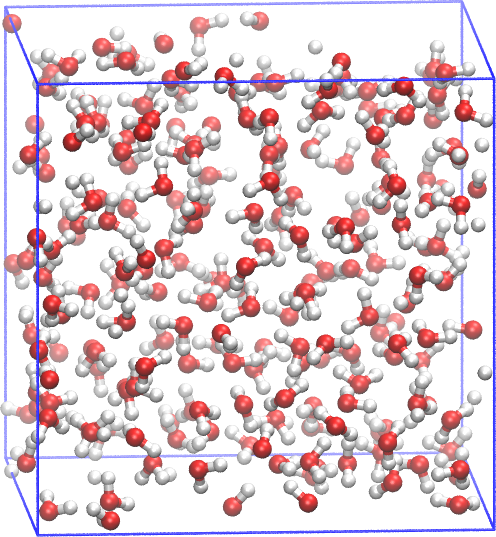
\includegraphics[height=1.45in,width=1.50in,viewport=0 0 140 138,clip]{Figures/Unit_Cell_of_Liquid_Water.png}
%\caption{\textrm{\tiny Schematic representation of water can be simulated using Periodic Boundary Conditions.}}
%\label{Water-PBC}
%\end{figure}
\begin{itemize}
\vspace{-8.0pt}
{\fontsize{9.5pt}{6.2pt}\selectfont{
	\item 基于\textrm{Boltzmann}分布,只能模拟平衡态体系
	\item 只计算势能(状态函数),不用计算力(瞬时作用)
\item 模拟步长可以比较大}}
\end{itemize}
\end{minipage}
\begin{minipage}{0.65\textwidth}
\begin{figure}[h!]
\centering
\vspace{-5.0pt}
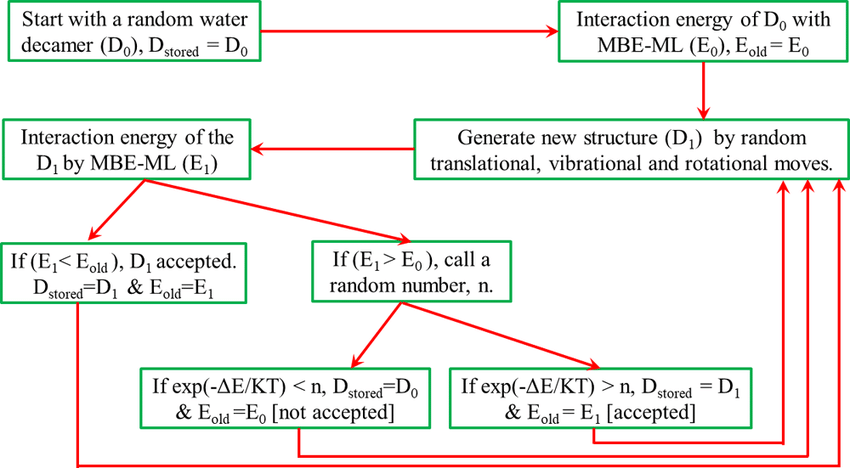
\includegraphics[height=1.55in,width=3.00in,viewport=0 0 930 475,clip]{Figures/Schematic-representation-of-the-Metropolis-Monte-Carlo-simulation.png}
%\caption{\textrm{Schematic representation of the Metropolis−Monte Carlo simulation.}}
\label{MC-Algorithm-Workflow}
\end{figure}
\end{minipage}
\begin{figure}[h!]
\centering
\vspace{-10.0pt}
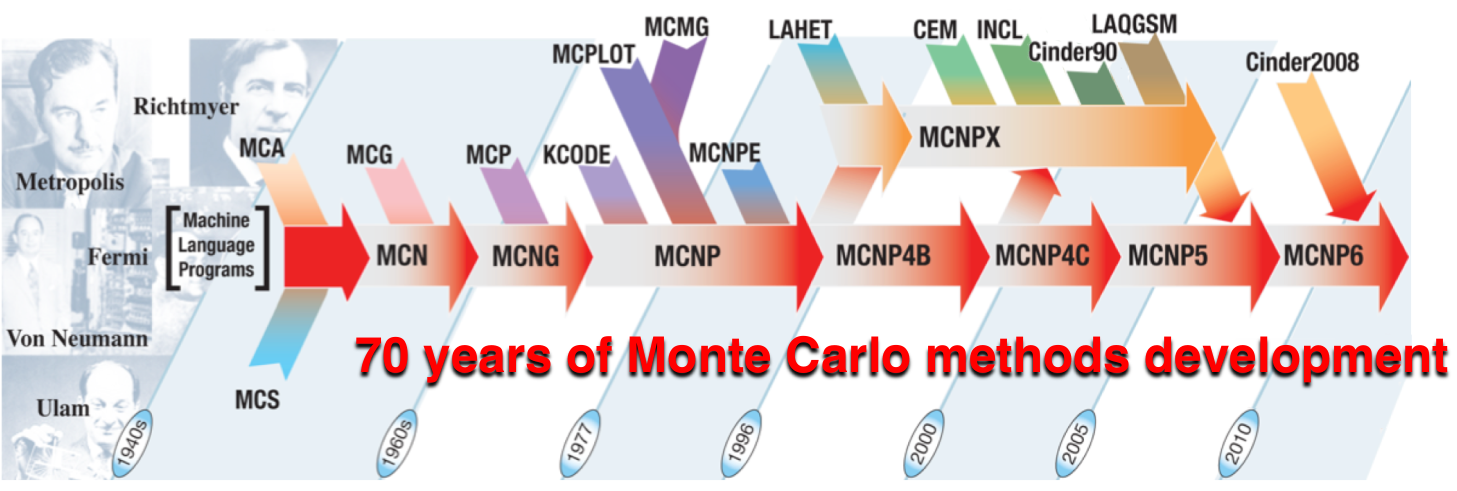
\includegraphics[height=1.25in,width=4.15in,viewport=0 0 1470 480,clip]{Figures/Monte-Carlo-development.png}
%\caption{\textrm{Schematic representation of the Metropolis−Monte Carlo simulation.}}
\label{Monte-Carlo-development}
\end{figure}
}

\subsection{经典分子动力学提要}
\frame
{
	\frametitle{}
\begin{figure}[h!]
\centering
\vspace{-7.0pt}
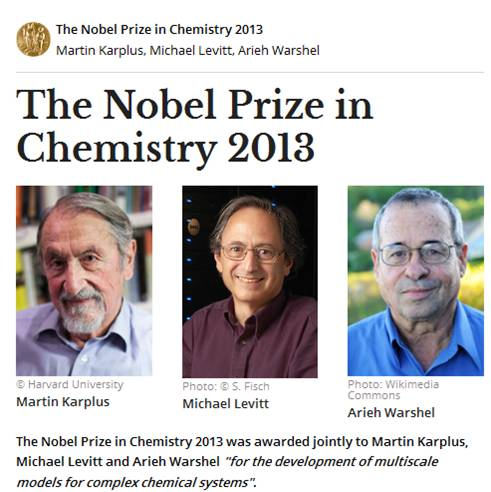
\includegraphics[height=2.85in,width=3.80in,viewport=0 0 410 300,clip]{Figures/Nobel_Prize_Chemistry-2013.jpg}
%\caption{\textrm{Schematic representation of the Metropolis−Monte Carlo simulation.}}
\label{Nobel-Prize-Chemistry_2013}
\end{figure}
}

\frame
{
	\frametitle{经典分子动力学}
\begin{minipage}{0.45\textwidth}
\begin{figure}[h!]
\centering
\vspace{-3.0pt}
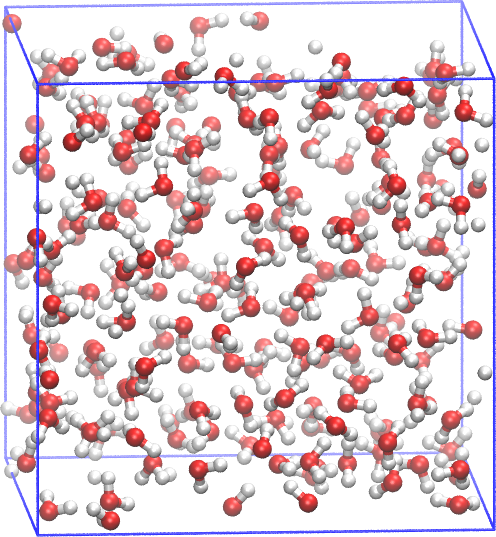
\includegraphics[height=2.00in,width=2.00in,viewport=0 0 135 135,clip]{Figures/Unit_Cell_of_Liquid_Water.png}
%\caption{\textrm{Schematic representation of the Metropolis−Monte Carlo simulation.}}
\label{Unit_Cell_of_Liquid_Water}
\end{figure}
\end{minipage}
\begin{minipage}{0.53\textwidth}
	\begin{itemize}
		\item 应用数值方法解析多粒子体系(原子、离子、$\cdots$)运动
		\item 粒子间相互作用可用简洁的解析函数或数值描述
		\item 广泛应用于材料科学、物理化学和生物科学的相关研究
		\item 模拟体系的粒子数规模:~\\$100\sim10^6$
		\item 模拟体系的时间范围:~\\$10~\mathrm{ps}\sim1\mu\mathrm{s}$~(一般是$\mathrm{ns}$范围)
	\end{itemize}
\end{minipage}
\begin{itemize}
	\item 分子动力学模拟可以包括温度和压力效应
	\item 分子动力学可以模拟相对大的体系和相对长的时间
	\item 分子动力学可以得到分子尺度的结构和动力学信息
\end{itemize}
}

\frame
{
	\frametitle{经典分子动力学}
	分子动力学方法的\textcolor{red}{优点}:
	\begin{itemize}
			\setlength{\itemsep}{5pt}
		\item 可以模拟大规模分子系统,原则上能计算系统的微观、宏观物理量,增补实验数据的空缺
		\item 与\textrm{Monte Carlo}方法相比,具备更高的准确度,可以提供更多微观粒子的运动细节
		\item 可以模拟非平衡态的体系以及体系在极端条件下复杂情况下的物理性质和物理状态
	\end{itemize}
	分子动力学方法的\textcolor{red}{缺点}:
	\begin{itemize}
			\setlength{\itemsep}{5pt}
		\item 只能描述原子(核)的运动,但无法反映电子的运动,难以准确模拟化学键
		\item 数值模拟依赖经验力场,化学环境复杂的体系,如化学键断裂,电子结构将由稳态电子结构过渡到过渡态,无法用简单的解析力场描述
	\end{itemize}
}

\frame
{
	\frametitle{相空间和时间平均}
	分子动力学模拟一般在相空间完成\\
	\vskip 3pt
	\textcolor{blue}{相空间}\textrm{(Phase~Space)}是表示系统所有可能所处状态的空间\\
	\vskip 5pt
{\fontsize{8.5pt}{6.2pt}\selectfont{
	\textcolor{blue}{系统中每个可能的状态在相空间中都存在一个确定的对应点}\\
	相空间是一个六维假想空间,其中\textcolor{blue}{动量}和\textcolor{blue}{空间}各占三维}}\\
	\vskip 8pt
	对于包含$N$个粒子的体系,构成$6N$维相空间$(\Gamma_N)$:~包括$3N$个空间$(\vec r)$自由度,$3N$个动量$(\vec p)$自由度
	\vskip 5pt
{\fontsize{8.2pt}{6.2pt}\selectfont{
	如果描述体系性质的状态函数$A$可以用空间和动量坐标表示~$A(\Gamma)$(如体系的总能或瞬时压力),其\textcolor{purple}{时间平均}值为}}
	\begin{displaymath}
		A_{\mathrm{obs}}=\langle A\rangle_{\mathrm{time}}=\langle A(\Gamma(t))\rangle_{\mathrm{time}}=\lim_{\tau\rightarrow\infty}\dfrac1{\tau}\int_{t=0}^{\tau}A(\Gamma(t))\mathrm{d}t
	\end{displaymath}
	\textcolor{magenta}{各态遍历假设}\textrm{(ergodic~hypothesis)}\\
	\vskip 5pt
{\fontsize{9.5pt}{6.2pt}\selectfont{
	只要演化时间足够长,孤立体系会\textcolor{red}{等概率地遍历每个可能的}微观状态~\\
换言之,\textcolor{blue}{体系足够长时间平均}等价于\textcolor{blue}{体系许可的大量系综的系综平均}
%分子动力学模拟的一个思想是用时间换取空间。我们无法得知系统在某一时刻所有可能的微观状态,但是可以通过一段时间的采样来获取系统大量的微观状态数。模拟的整个过程可以理解为建立了一个系综,而每一个时间点就是组成这个系综的一个系统,它们具有相同的限制条件(例如:粒子总数,温度、压强或体积等),但是具有不同的微观状态。系统的热力学量就是系综平均的结果。
}}
}

\frame
{
	\frametitle{分子动力学基本思想}
	\begin{itemize}
			\setlength{\itemsep}{3pt}
		\item 分子动力学模拟过程中产生的具体数据是\\
			\textcolor{blue}{粒子在相空间中随时间演化的 一系列点}
		\item 分子动力学模拟的直接结果是\\
			\textcolor{blue}{体系中全部粒子随时间变化的径迹\textrm{(trajectory)}}
		\item 体系的时间平均和其它物理性质都可以通过粒子径迹计算
		\item 约化单位\textrm{(reduced unit)}\\
{\fontsize{7.2pt}{6.2pt}\selectfont{
	数值模拟中使用的是内部单位,需要通过换算才能得到实际体系的真实物理单位(国际单位制,\textrm{Syst\`eme International $\mathrm{d}'$Unit\'es, SI})}}
	\begin{enumerate}
{\fontsize{7.2pt}{6.2pt}\selectfont{
		\item 四个基本物理量单位:\\
			长度\textrm{L}、质量\textrm{M}、时间\textrm{t},电荷电量\textrm{Q}
		\item 其它物理量:\\
			能量~$E=M\cdot L^2/t^2$\hskip 15pt温度~$T=E/k_{\mathrm{B}}$\hskip 15pt压力~$P=E/L^3$\\
			质量密度~$\rho=M/L^3$\hskip 8pt数量密度~$n=1/L^3$\hskip 8pt介电常数~$\varepsilon=\dfrac{N_{\mathrm{A}}\cdot Q^2}{L\cdot E}$
			\vskip 4pt
	这里$k_{\mathrm{B}}$是\textrm{Boltzmann}常数,$N_{\mathrm{A}}$是\textrm{Avogadro}常数}}
	\end{enumerate}
	\end{itemize}
}

\frame
{
	\frametitle{分子动力学基本思想}
	在相空间中,体系中粒子的运动由\textrm{Hamiltonian}方程描述
	\begin{displaymath}
		\begin{aligned}
			\dot{\vec r}_i=&\dfrac{\partial\mathbf{H}}{\partial\vec p_i}=\dfrac{\vec p_i}{m_i}\\
			\dot{\vec p}_i=&-\dfrac{\partial\mathbf{H}}{\partial\vec r_i}=\vec f_i
		\end{aligned}
	\end{displaymath}
	\textrm{Hamiltonian}$\mathbf{H}$的定义为
	\begin{displaymath}
		\begin{aligned}
			\mathbf{H}(\vec r,\vec p)=&\mathbf{K}(\vec p)+V(\vec r)\\
			\mathbf{K}(\vec p)=&\sum_i^N\dfrac{\vec p_i^2}{2m_i}
		\end{aligned}
	\end{displaymath}
	由此可得粒子运动遵守的\textrm{Newton}方程为
	\begin{displaymath}
		\begin{aligned}
			\dot{\vec x}=&\dfrac{\partial\mathbf{H}}{\partial\vec p_x}=\dfrac{\vec p_x}m=\vec v_x\\
			\dot{\vec p}_x=&-\dfrac{\partial\mathbf{H}}{\partial{\vec x}}=-\dfrac{\partial V(\vec x)}{\partial\vec x}=\vec F=m\vec a_x
		\end{aligned}
	\end{displaymath}
}

\frame
{
	\frametitle{分子动力学模拟流程}
\begin{figure}[h!]
\centering
\vspace{-10.0pt}
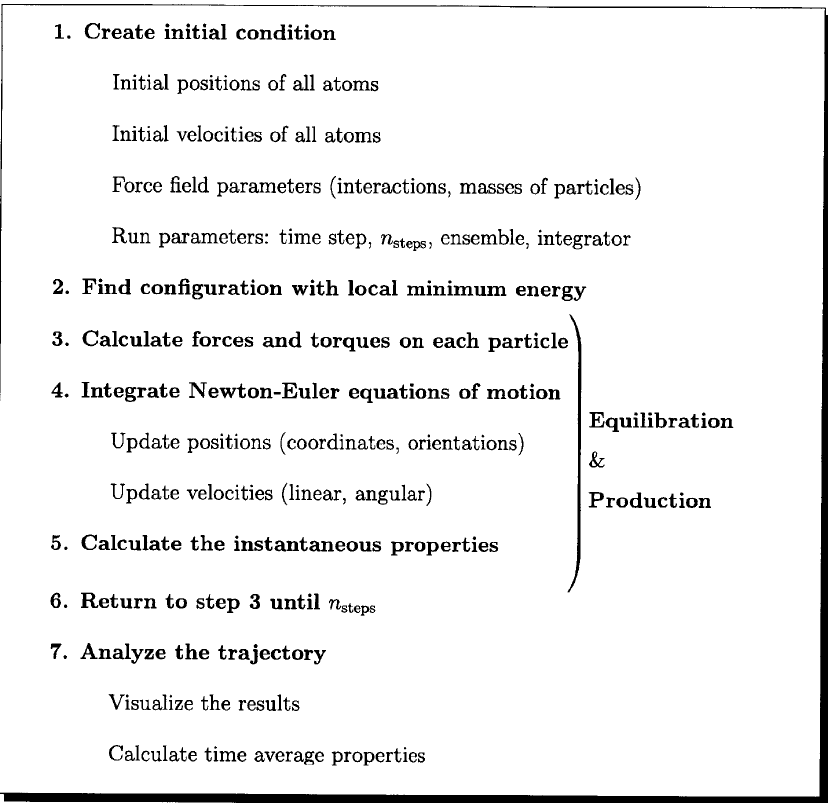
\includegraphics[height=2.70in,width=3.00in,viewport=30 20 750 794,clip]{Figures/The-molecular_dynamcis_algorithm.png}
\caption{\textrm{The steps in performing a molecular dynamcis simulation.}}
\label{The-molecular-dynamics_algorithm}
\end{figure}
}

\subsection{分子动力学的力场}
\frame[allowframebreaks]
{
	\frametitle{力场}
分子动力学中,粒子间相互作用用\textcolor{red}{力场}\textrm{(Force Field)},也就是“\textcolor{blue}{相互作用势}”,描述,力场的形式有很多种,一般将势函数分解为粒子间相互作用,包括双体相互作用、三体相互作用、$\cdots$
	\begin{displaymath}
		V(\vec r)=\sum_{ij}V_{ij}(\vec r_i,\vec r_j)+V_{ijk}(\vec r_i,\vec r_j,\vec r_k)+V_{ijkl}(\vec r_i,\vec r_j,\vec r_k,\vec r_l)+\cdots
	\end{displaymath}
\begin{figure}[h!]
\centering
\vspace{-18.0pt}
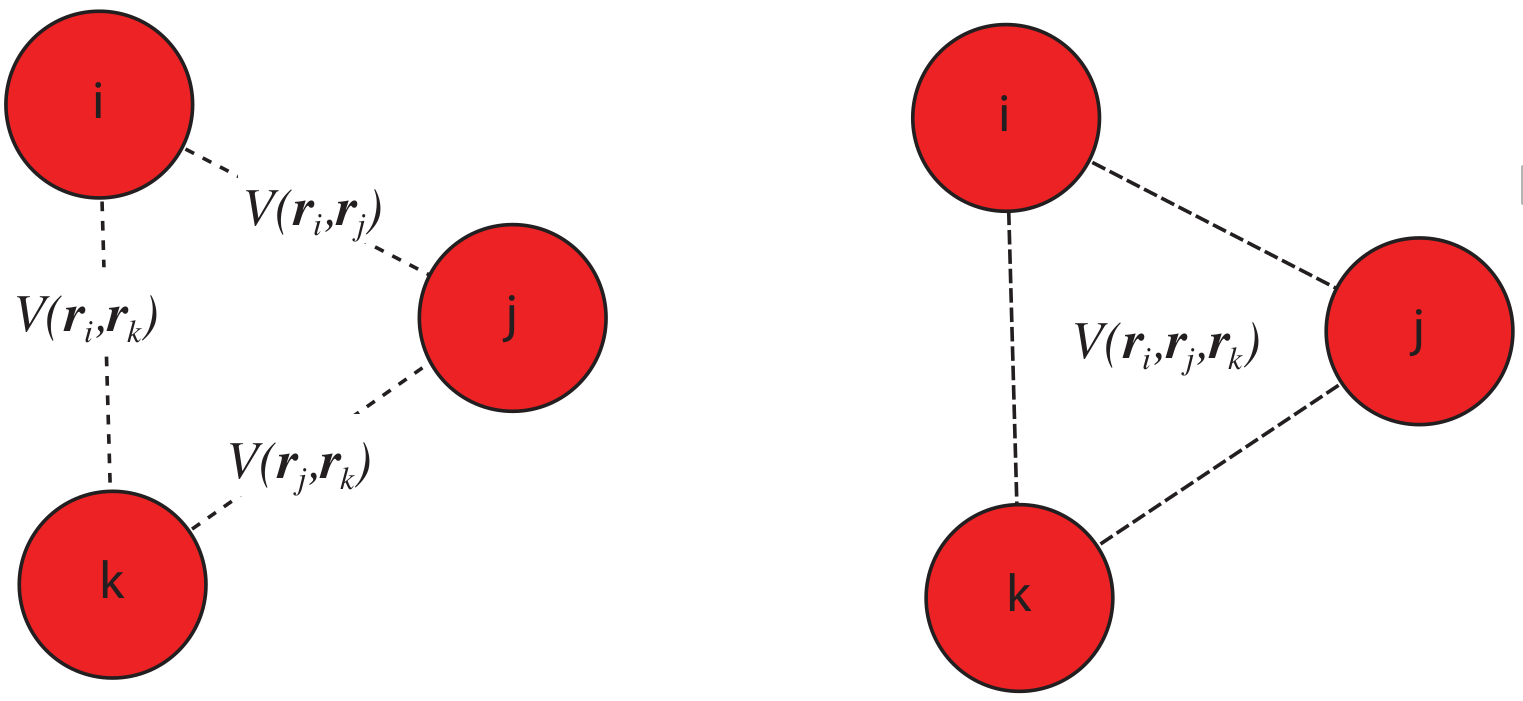
\includegraphics[height=1.47in,width=3.40in,viewport=0 0 1520 700,clip]{Figures/Interaction_particles.png}
\caption{\textrm{\tiny The Schematic representation of the interactions between pairs, triplets of particles.}}
\label{Interaction_particles}
\end{figure}

\begin{itemize}
			\setlength{\itemsep}{5pt}
	\item 一般说,力场中最主要来自双体相互作用(也称为``对势''),因此可将力场展开函数中的多体相互作用截断,仅保留双体相互作用的贡献
		\begin{displaymath}
			V(\vec r)=\sum_{ij}V_{ij}(\vec r_i,\vec r_j)
		\end{displaymath}
	\item 真实模拟中,为了更好地表示考虑粒子间相互作用的多体效应,双体相互作用用的是``有效对势'',有效对势包含了一部分粒子间的多体相互作用
		\begin{displaymath}
			V(\vec r)=\sum_{ij}V_{ij}^{\mathrm{eff}}(\vec r_i,\vec r_j)
		\end{displaymath}
	\item 具体计算使用的力场都是参数化的,这些参数主要通过对实验数据和结果的拟合确定
\end{itemize}

	典型力场的有
	\begin{itemize}
		\item \textrm{Lennard-Jones}对势和受力
	\begin{displaymath}
		\begin{aligned}
			U(r)=&4\varepsilon\bigg[\bigg(\dfrac{\sigma}{r}\bigg)^{12}-\bigg(\dfrac{\sigma}{r}\bigg)^6\bigg]\\ 
			\vec F(r)=&-\nabla V(r)=24\dfrac{\varepsilon}r\bigg[2\bigg(\dfrac{\sigma}{r}\bigg)^{12}-\bigg(\dfrac{\sigma}{r}\bigg)^6\bigg]\hat{\vec r}
		\end{aligned}
	\end{displaymath}
	{\fontsize{7.2pt}{6.2pt}\selectfont{这里$\varepsilon$和$\sigma$是和原子有关的参数}}
		\begin{itemize}{\fontsize{8.0pt}{6.2pt}\selectfont{
			\item \textcolor{blue}{$\dfrac1{r^6}$项}:~描述中性原子间的\textrm{Vander-der-Waals}的相互吸引作用(包含偶极-偶极相互作用)
			\item \textcolor{blue}{$\dfrac1{r^{12}}$项}:~描述电子云重叠引起的短程排斥作用
			\item \textrm{L-J}势能的最低点在$r_{\min}=2^{(1/6)}\sigma\approx1.122\sigma$\\
				$r<r_{\min}$时为排斥力,$r>r_{\min}$时为吸引力}}
		\end{itemize}
惰性气体的原子间相互作用仅用\textrm{L-J}基本可以完全描述
\begin{figure}[h!]
\centering
\vspace*{-0.15in}
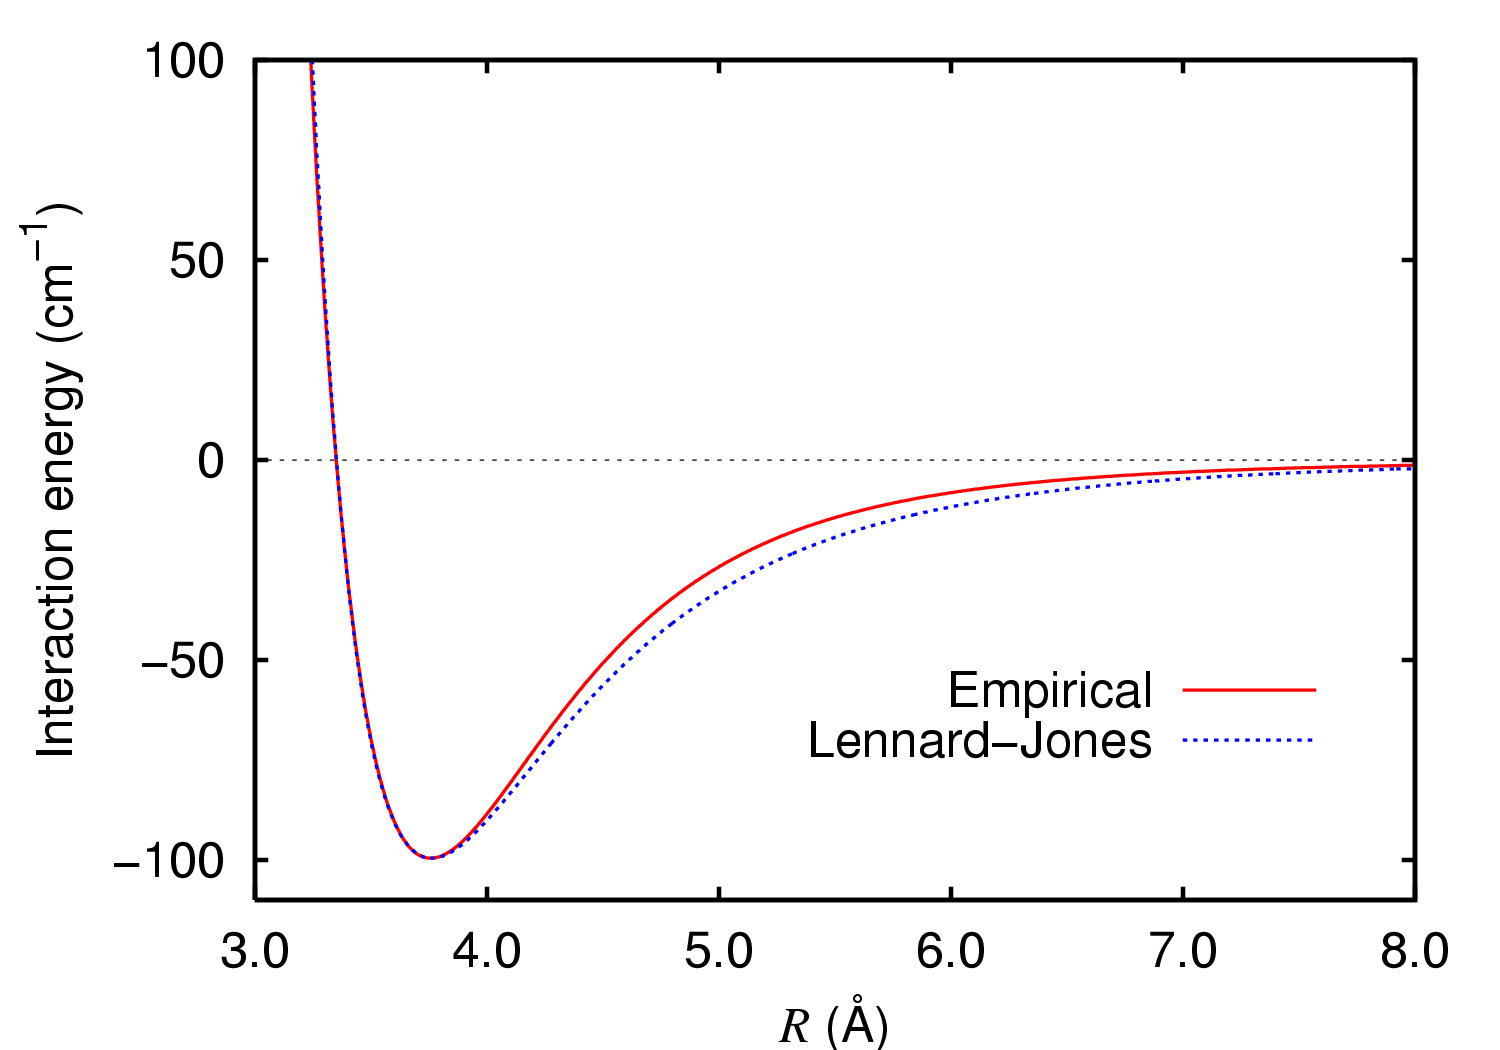
\includegraphics[height=2.05in,width=2.90in,viewport=0 0 350 270,clip]{Figures/Argon_dimer_potential_and_Lennard-Jones.png}
\caption{\tiny \textrm{The Lennard-Jones potential for argon dimer.}}%(与文献\cite{EPJB33-47_2003}图1对比)
\label{Potential-Lennard-Jones}
\end{figure}
%	由\textrm{L-J}势改造,可以得到\textrm{WCA}势和\textrm{PHS}势
\item \textrm{Morse}势
	\begin{displaymath}
		U(r)=-D_{\mathrm{e}}+D_{\mathrm{e}}\bigg(1-\mathrm{e}^{-a(r-r_{\mathrm{e}})}\bigg)^2
	\end{displaymath}
	{\fontsize{6.5pt}{6.2pt}\selectfont{这里$D_{\mathrm{e}}$是\textrm{Morse}势的势阱深,参数$a$确定势阱宽度,$r_{\mathrm{e}}$是原子处于平衡位置的平衡键长 }}
\begin{figure}[h!]
\centering
\vspace*{-0.10in}
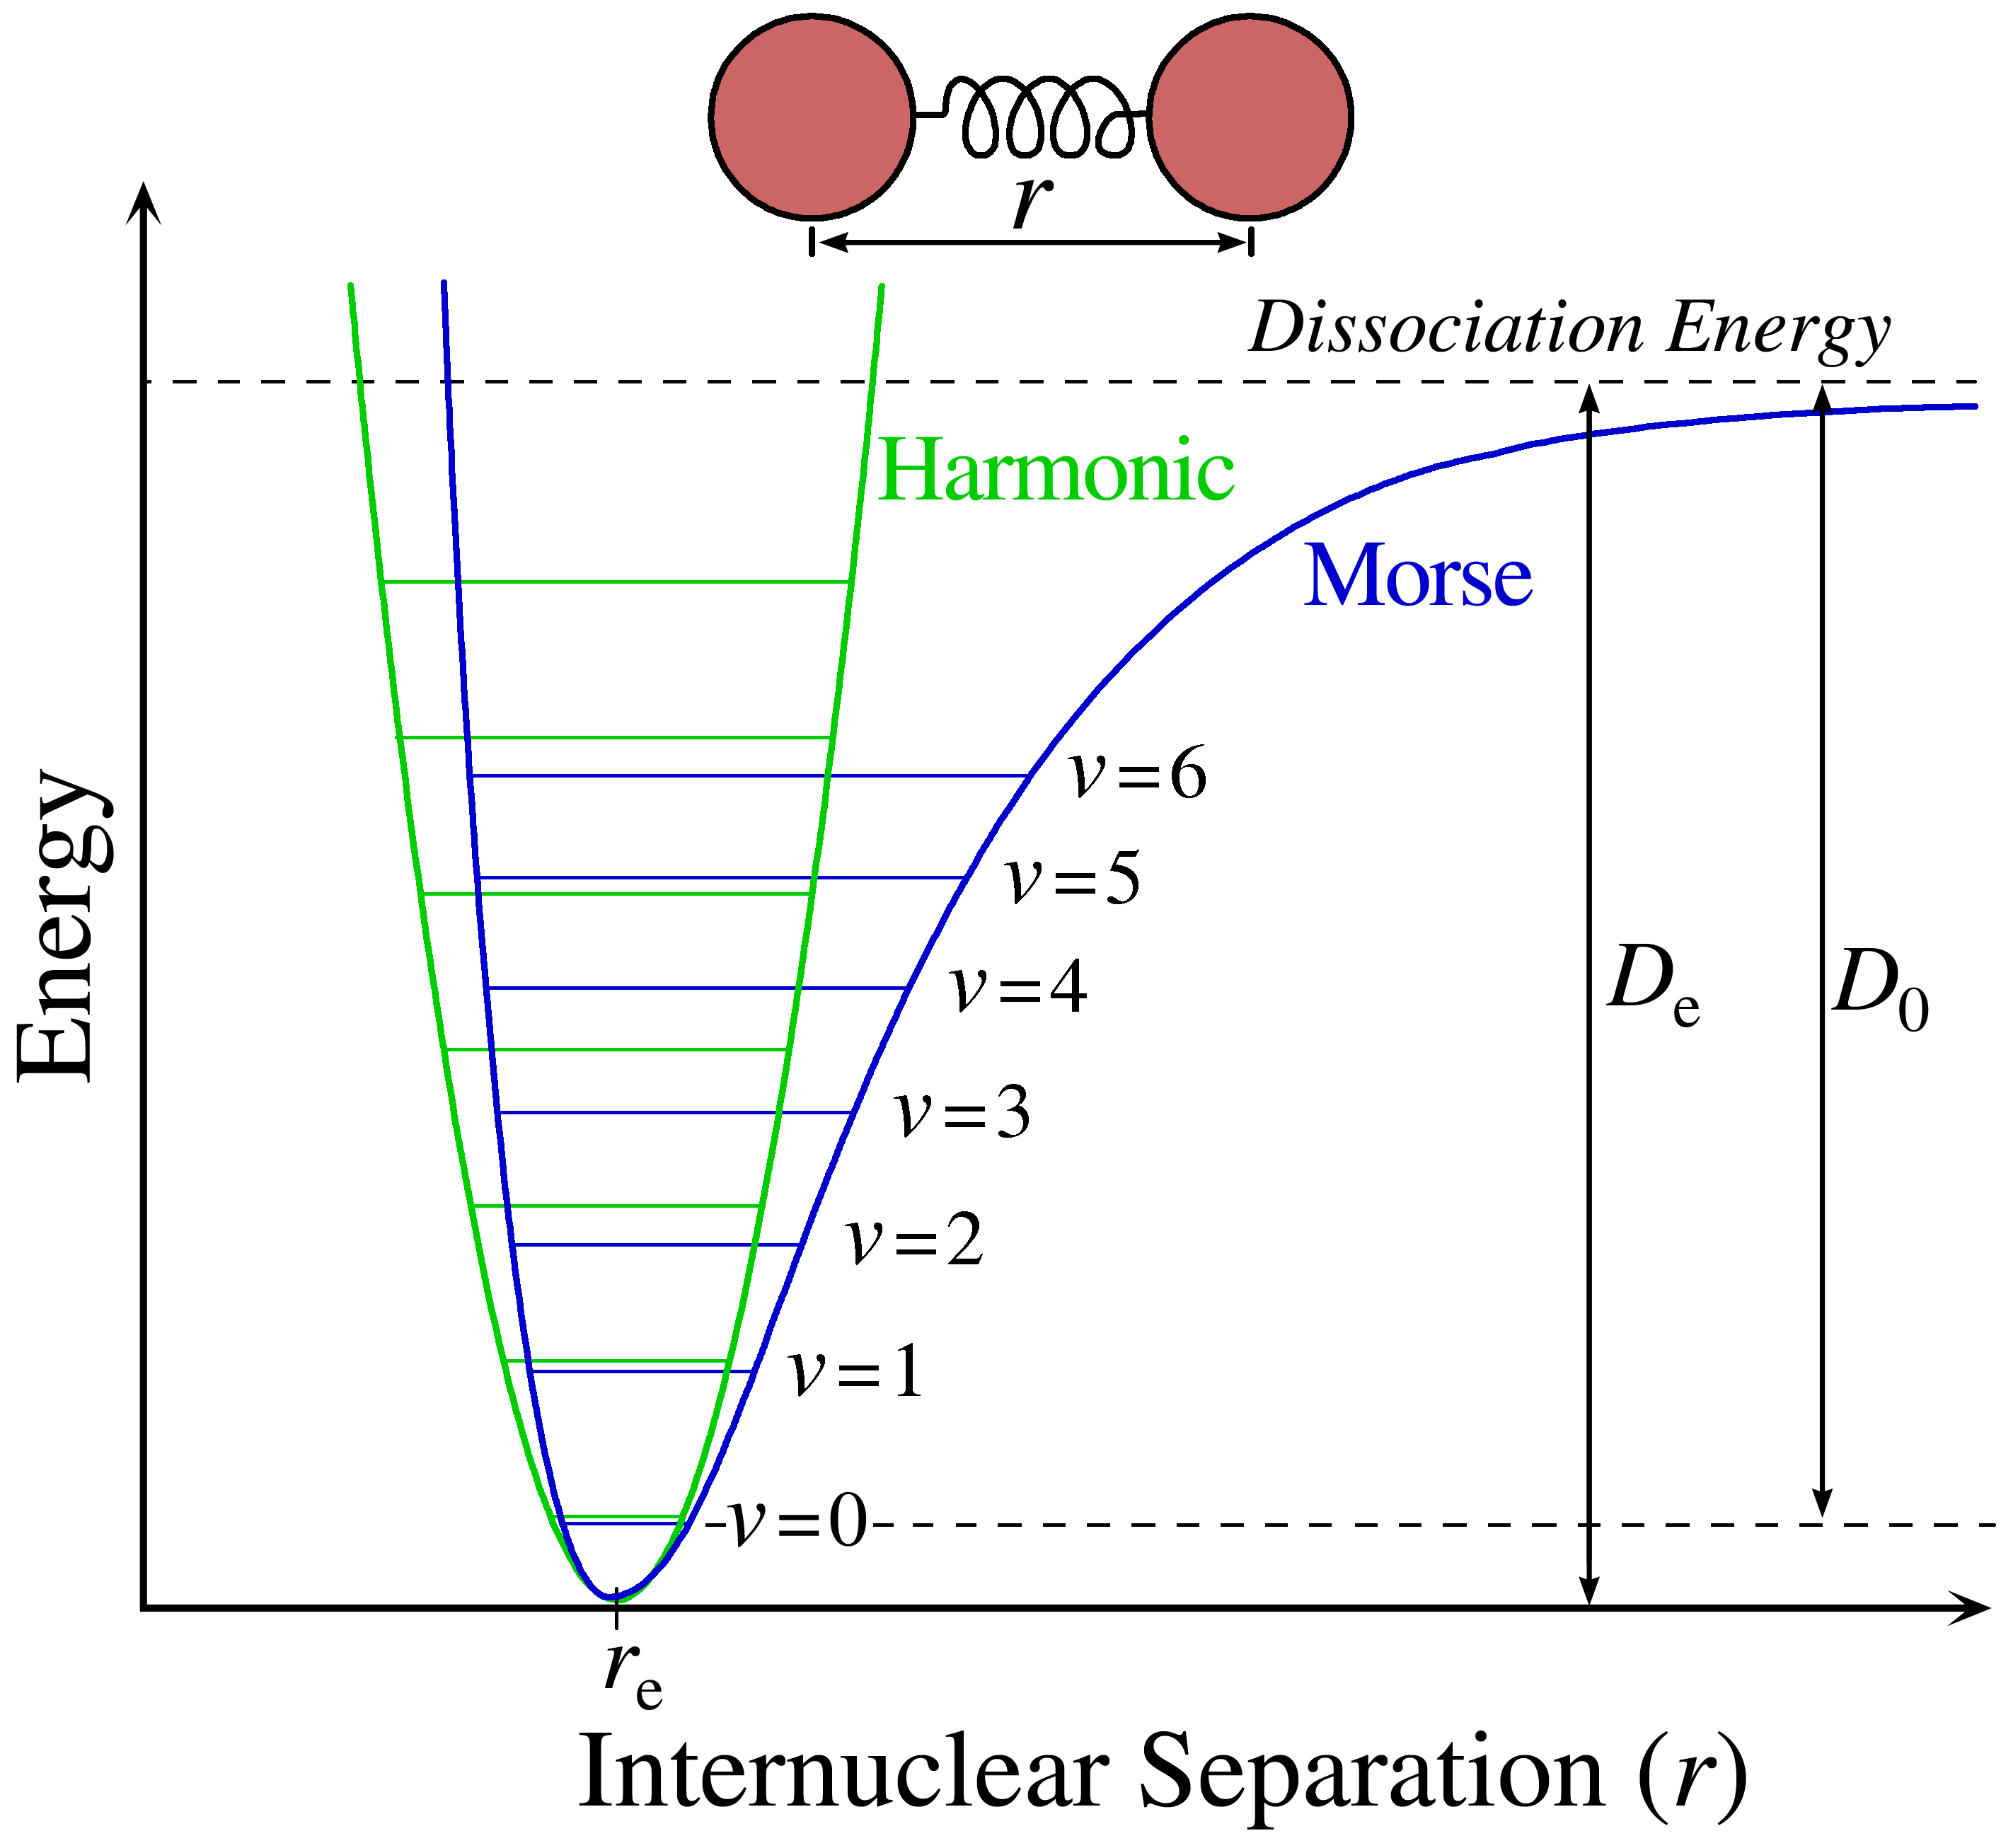
\includegraphics[height=1.35in,width=1.95in,viewport=0 0 3540 2770,clip]{Figures/Morse-potential.png}
\caption{\tiny \textrm{The Morse potential (blue) and harmonic oscillator potential (green).}}%(与文献\cite{EPJB33-47_2003}图1对比)
\label{Potential-Morse}
\end{figure}
\item \textrm{EAM}势\\
	{\fontsize{7.2pt}{6.2pt}\selectfont{对于金属晶体,内能虽可以表示为对相互作用之和,但拟合原子受力非常困难:\footnote{\fontsize{5.2pt}{3.2pt}\selectfont{应用二体势计算金属弹性常数时必须涉及对体积很敏感的能量项,因为涉及缺陷、表面的体积很难确定。}}\\
	\textcolor{red}{从物理上说金属原子处于电子海洋中,电子密度来自多个原子的贡献,这是自由电子气带来的多体效应}}}\\
	\textrm{EAM}将金属中原子的势能表示为二体势和多体势之和
	\begin{displaymath}
		E_i=F_{\alpha}\bigg(\sum_{j\neq i}\rho_{\beta}(r_{ij})\bigg)+\dfrac12\sum_{j\neq i}\phi_{\alpha\beta}(\vec r_{ij})
	\end{displaymath}
	{\fontsize{7.2pt}{6.2pt}\selectfont{$\alpha$和$\beta$分别为位置$i$、$j$处的原子类型\\
		$\phi$是二体势,是原子$\alpha$和$\beta$和原子间距$r_{ij}$的函数\\
		$F$是多体势,是其余原子在位置$i$处的电荷密度与位置$i$处原子$\alpha$的相互作用能,由原子类型$\alpha$和位置$i$处的电子密度确定\\
		位置$j$原子在位置$i$处产生的电荷密度$\rho$只与位置$j$处原子类型$\beta$和原子间距$r_{ij}$有关,与方向无关
	}}\\
	各类\textrm{EAM}势中,$\phi(r)$、$\rho(r)$和$F(\rho)$都不是解析的,以数值形式存储
	\end{itemize}
}

\frame
{
	\frametitle{复杂研究对象中的力场}
\begin{figure}[h!]
\centering
\vspace*{-0.10in}
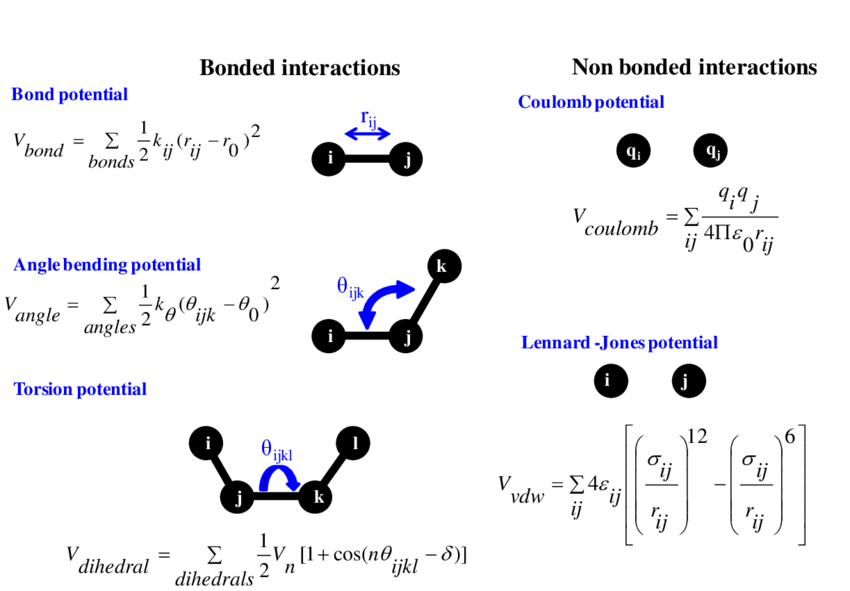
\includegraphics[height=2.70in,width=3.95in,viewport=0 0 830 550,clip]{Figures/Bonded-and-non-bonded-interactions-used-to-describe-interactions-between-atoms.png}
%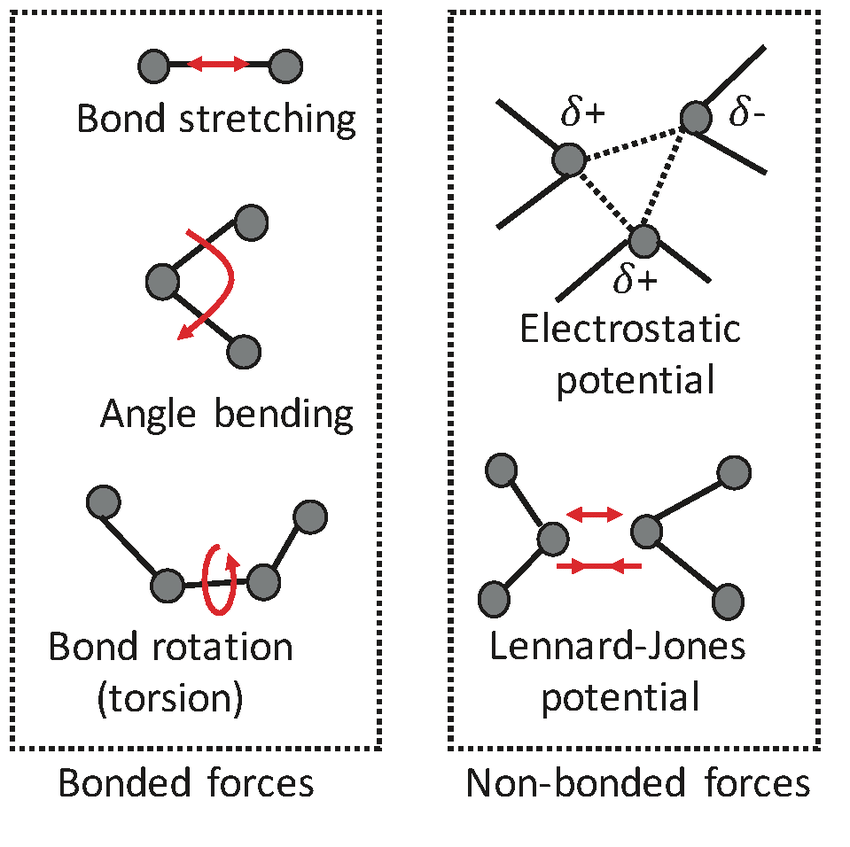
\includegraphics[height=2.70in,width=2.85in,viewport=0 40 830 850,clip]{Figures/Bonded-and-non-bonded-forces-consider-in-MD-simulations.png}
\caption{\tiny \textrm{Bonded and non-bonded forces consider in MD simulations.}}%(与文献\cite{EPJB33-47_2003}图1对比)
\label{Bond-non-Bonded}
\end{figure}
}

\frame
{
	\frametitle{复杂研究对象中的力场}
\begin{figure}[h!]
\centering
\vspace*{-0.15in}
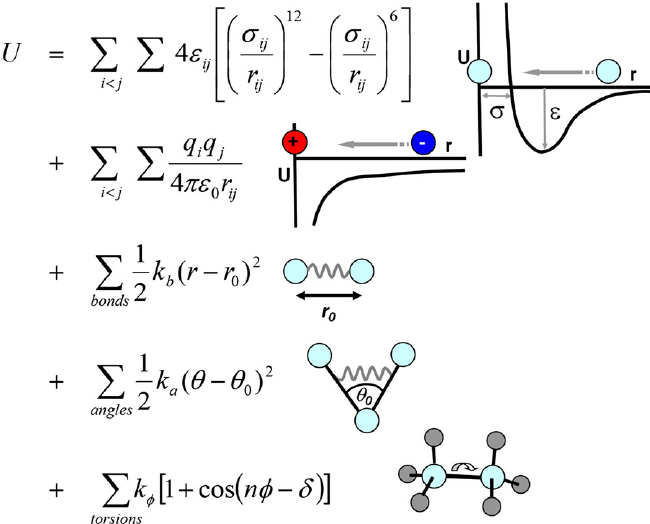
\includegraphics[height=2.75in,width=3.55in,viewport=0 0 660 540,clip]{Figures/Potential-energy-function-for-molecular-interactions-in-the-molecular-mechanics.png}
\caption{\tiny \textrm{Potential energy function for molecular interactions in the molecular mechanics.}}%(与文献\cite{EPJB33-47_2003}图1对比)
\label{Potential-component}
\end{figure}
}

\subsection{分子动力学\rm{Verlet}算法}
\frame
{
	\frametitle{分子的受力与运动}
	装有$N$个经典粒子的$L_1\times L_2\times L_3$容器内,假设粒子间只有简单的二体相互作用%\footnote{\fontsize{7.2pt}{6.2pt}\selectfont{二体作用是粒子间多体相互作用的简化,只考虑粒子两两间彼此相互作用。}}
	$\vec F(r)$,力的大小仅与粒子间间距$r$相关
	\begin{displaymath}
		\vec F(R_i)=\sum_{\substack{j=1\\j\neq i}}^N F(|\vec r_i-\vec r_j|)\hat{\vec r}_{ij}
	\end{displaymath}
	{\fontsize{7.2pt}{6.2pt}\selectfont{这里$R$代表全部原子坐标$\vec r_i$,$\hat{\vec r}_{ij}$是表示粒子$i$指向粒子$j$的矢量($\vec r_j-\vec r_i$)的单位矢量}}

	在经典力学框架下,粒子$i$的受力运动方程是:~
	\begin{displaymath}
		\dfrac{\mathrm{d}^2\vec r_i(t)}{\mathrm{d}t^2}=\dfrac{\vec F_i(R)}{m_i}
	\end{displaymath}
	粒子$i$的质量是$m_i$\\
	\textcolor{purple}{经典分子动力学,就是应用数值模拟对大量粒子求解该方程,基于统计力学原理,研究物质的状态和热力学性质}
}

\frame
{
	\frametitle{经典分子动力学与\textrm{Verlet}算法}
	分子动力学模拟研究的对象是平衡态体系
	\begin{itemize}
		\item 初始化
		\item 开始分子运动模拟,直到模拟体系达到平衡
		\item 继续模拟体系的物理性质,保存计算结果
	\end{itemize}
	\textcolor{blue}{标准\textrm{Verlet}算法:~}求解作用力$\vec F$下单个粒子运动的积分
	\begin{displaymath}
		\vec r(t+h)=2\vec r(t)-\vec r(t-h)+h^2\vec F(\vec r(t))/m
	\end{displaymath}
	{\fontsize{7.2pt}{6.2pt}\selectfont{这里$h$是时间步长,$t=nh$是模拟累积时间,$\vec r(t)$是粒子在时间$t$时的位置\\
	\textcolor{magenta}{每个时间步长的误差为$h^4$,在模拟时间范围内的累积误差是$h^2$}
\vskip 5pt
	{\fontsize{7.2pt}{6.2pt}\selectfont{如果已知模拟粒子的初始速度$\vec v$和时间,取初始态时间$t=0$}}
	\begin{displaymath}
		\vec r(h)=\vec r(0)=h\vec v(0)+\dfrac{h^2}2\vec F[\vec r(t=0)]~\qquad~ (m\equiv1)
	\end{displaymath}
误差为$h^3$,速度随时间变化的函数
\begin{displaymath}
	\vec v(t)=\dfrac{\vec r(t+h)-\vec r(t-h)}{2h}+\mathscr{O}(h^2)
\end{displaymath}
}}
}

\frame
{
	\frametitle{经典分子动力学与\textrm{Verlet}算法}
	\textrm{Verlet}算法有两种被普遍应用的变体形式,相比于标准\textrm{Verlet}算法,这两种方法误差累积效应更小
	\begin{itemize}
		\item \textcolor{blue}{蛙跳(\textrm{Leap-Frog})法}
			\begin{displaymath}
				\begin{aligned}
					\vec v(t+h/2)=&\vec v(t-h/2)+h\vec F[\vec r(t)]\\
					\vec r(t+h)=&\vec r(t)+h\vec v(t+h/2)
				\end{aligned}
			\end{displaymath}
		\item \textcolor{blue}{速度-\textrm{Verlet}算法}
			\begin{displaymath}
				\vec v(t)=\dfrac{\vec r(t+h)-\vec r(t-h)}{2h}
			\end{displaymath}
			\begin{displaymath}
				\begin{aligned}
					\vec r(t+h)=&\vec r(t)+h\vec v(t)+h^2\vec F(t)/2\\
					\vec v(r+h)=&\vec v(t)+h[\vec F(t+h)+\vec F(t)]/2
				\end{aligned}
			\end{displaymath}
			速度-\textrm{Verlet}算法更稳定也更方便,但需要保存$\vec F(t)$和$\vec F(t+h)$两个力的数组
	\end{itemize}
}

\frame
{
	\frametitle{经典分子动力学与\textrm{Verlet}算法}
	以下算法与速度-\textrm{Verlet}算法完全等价,但只需要保留$\vec F(t)$一个数组
	\begin{displaymath}
		\begin{aligned}
			\tilde{\vec v}(t)=&\vec v(t)+h\vec F(t)/2\\
			\vec r(t+h)=&\vec r(t)+h\tilde{\vec v}(t)\\
			\vec v(t+h)=&\tilde{\vec v}(t)+h\vec F(t+h)/2
		\end{aligned}
	\end{displaymath}
	而粒子受力$\vec F(t+h)$则在第二步、第三步之间临时计算
\vskip 5pt
	{\fontsize{6.2pt}{4.2pt}\selectfont{一般地,作用在粒子$i$上的力,是所有与粒子$i$的相互作用的“合成”结果
	\begin{displaymath}
		\vec F_i(R)=-\dfrac{\partial U(\{\vec r_i\})}{\partial \vec r_i}
	\end{displaymath}
	通常总的势能$U(\{\vec r_i\})$拆解为各部分贡献
	\begin{displaymath}
		U(\{\vec r_i\})=\sum_iU_1(\vec r_i)+\sum_i\sum_{j>i}U_2(\vec r_i,\vec r_j)+\sum_i\sum_{j>i}\sum_{k>j}U_3(\vec r_i,\vec r_j,\vec r_k)+\cdots
	\end{displaymath}
	这里$U_1(\vec r_i)$是单体势,一般是单个粒子在外场(如重力场、电场)中的势能,与材料性质无关\\
$U_2(\vec r_i,\vec r_j)$是双体势,$U_3(\vec r_i,\vec r_j,\vec r_k)$是描述粒子间对相互作用的主要函数}}

	在分子动力学计算中,力的计算需要更多的时间,因为其计算耗时步数是$\mathscr{O}(N^2)$,\textcolor{blue}{对于周期体系,这种力的计算尤其需要谨慎}
}

\subsection{平衡态统计基础}
\frame
{
	\frametitle{平衡态统计基础}
	系综(\textrm{Ensembles})是在一定的宏观条件下,由大量微观粒子组成的性质和结构完全相同的、处于各种运动状态的、各自独立的系统整体的集合。简言之,系综是给定宏观条件下,所有微观状态的集合。
%	应用\textrm{Verlet}算法,完成单粒子运动的数值积分,可以得到动力学体系的\textrm{Hamiltonian}对应的能量,进而应用统计力学的统计系综,获得宏观体系的物理量
	\vskip 3pt
	\textcolor{blue}{等概率原理}\textrm{(Principle of equal weights)}:\\
	一个热力学体系有相同的概率到达每个可能经历的微观态。\\
	等概率原理导出\textrm{Boltzmann}分布
	\begin{displaymath}
		P_j=\dfrac{\mathrm{e}^{-\beta\varepsilon_j}}Q
	\end{displaymath}
	这里$Q$称为配分函数\textrm{(partition function)}
	\begin{displaymath}
		\begin{aligned}
			Q=&\sum_i\mathrm{e}^{(-\beta\varepsilon_i)}\\
			\beta=&1/k_{\mathrm{B}}T
		\end{aligned}
	\end{displaymath}
	物理量的系综平均
	\begin{displaymath}
		\langle A\rangle=\sum_jA_j\mathrm{e}^{(-\beta\varepsilon_j)}/Q
	\end{displaymath}
}

\frame
{
	\frametitle{常用统计系综}
\begin{figure}[h!]
\centering
\vspace*{-0.20in}
%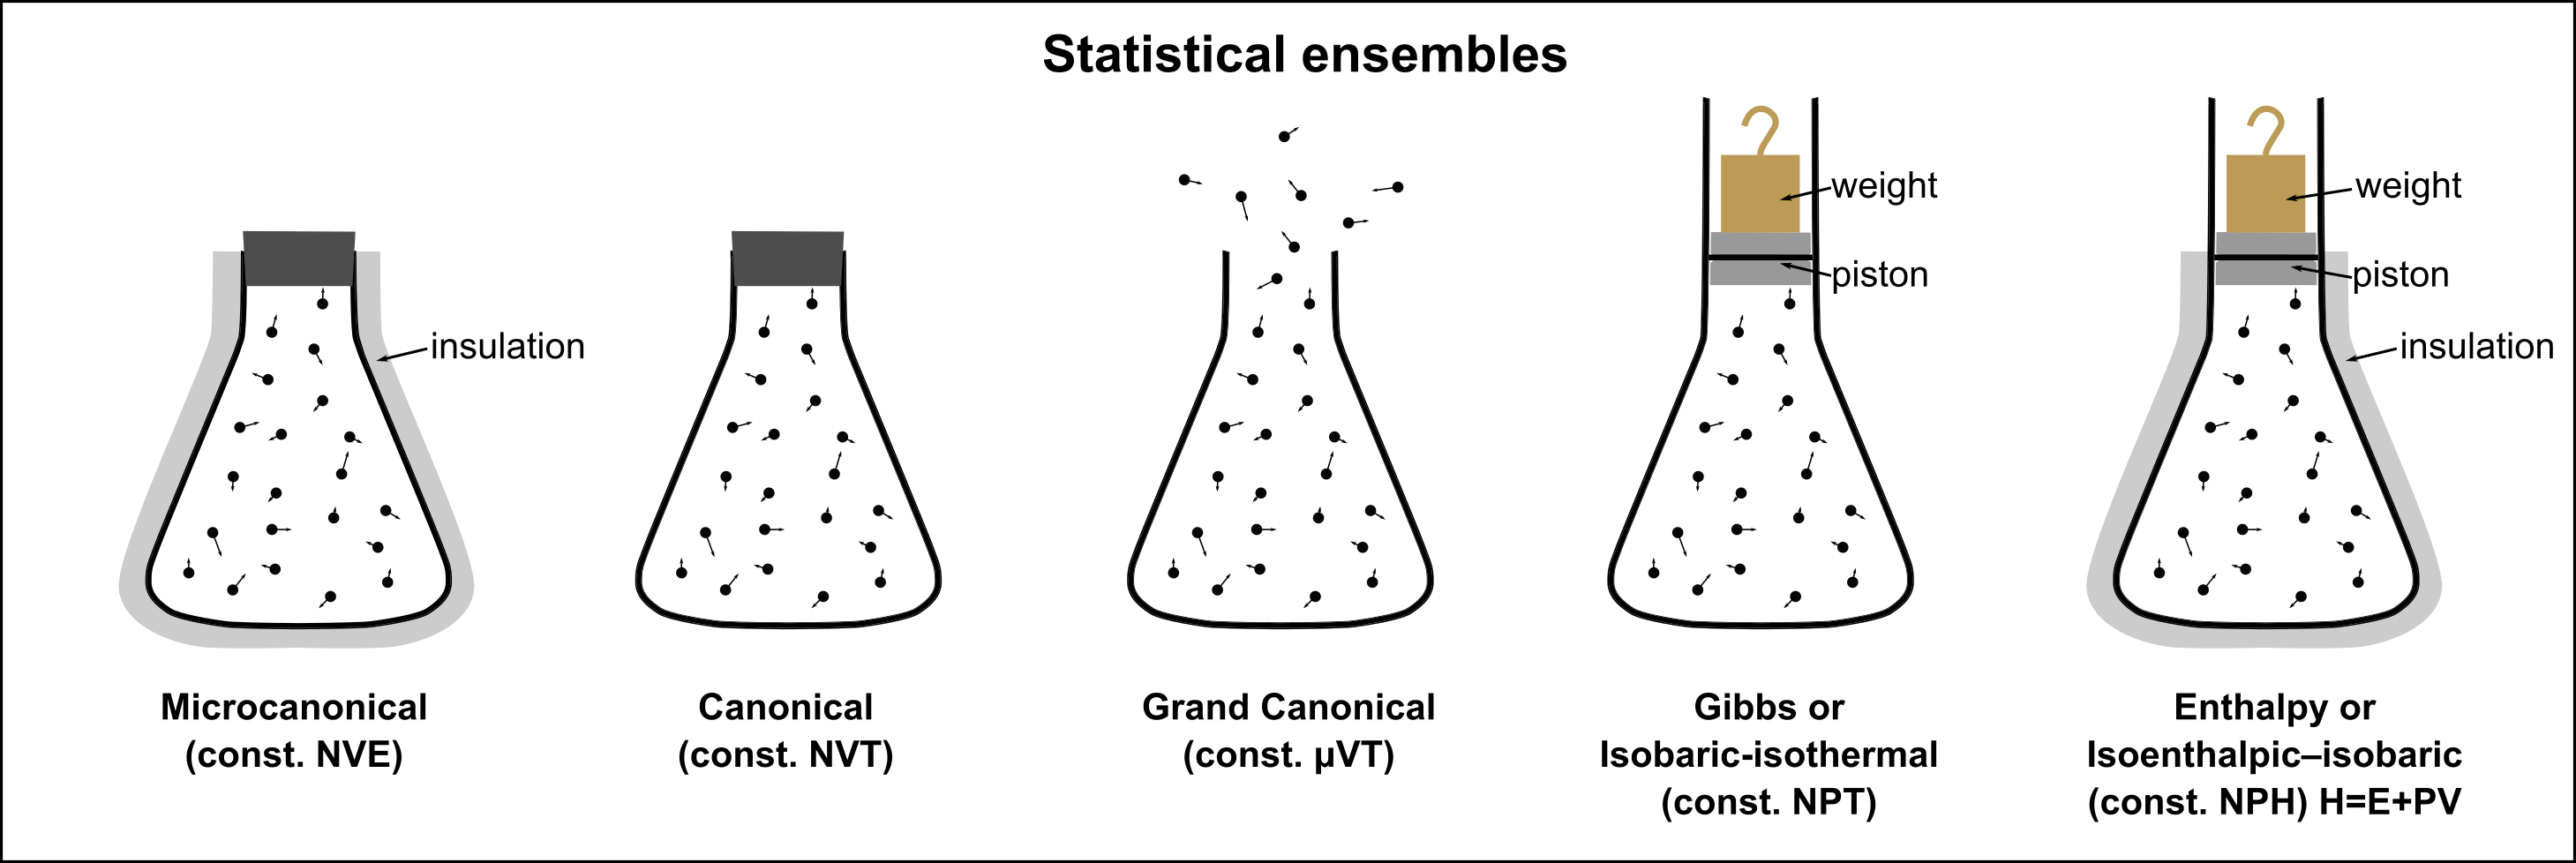
\includegraphics[height=1.60in,width=3.85in,viewport=0 0 1420 570,clip]{Figures/Statistical_Ensembles.png}
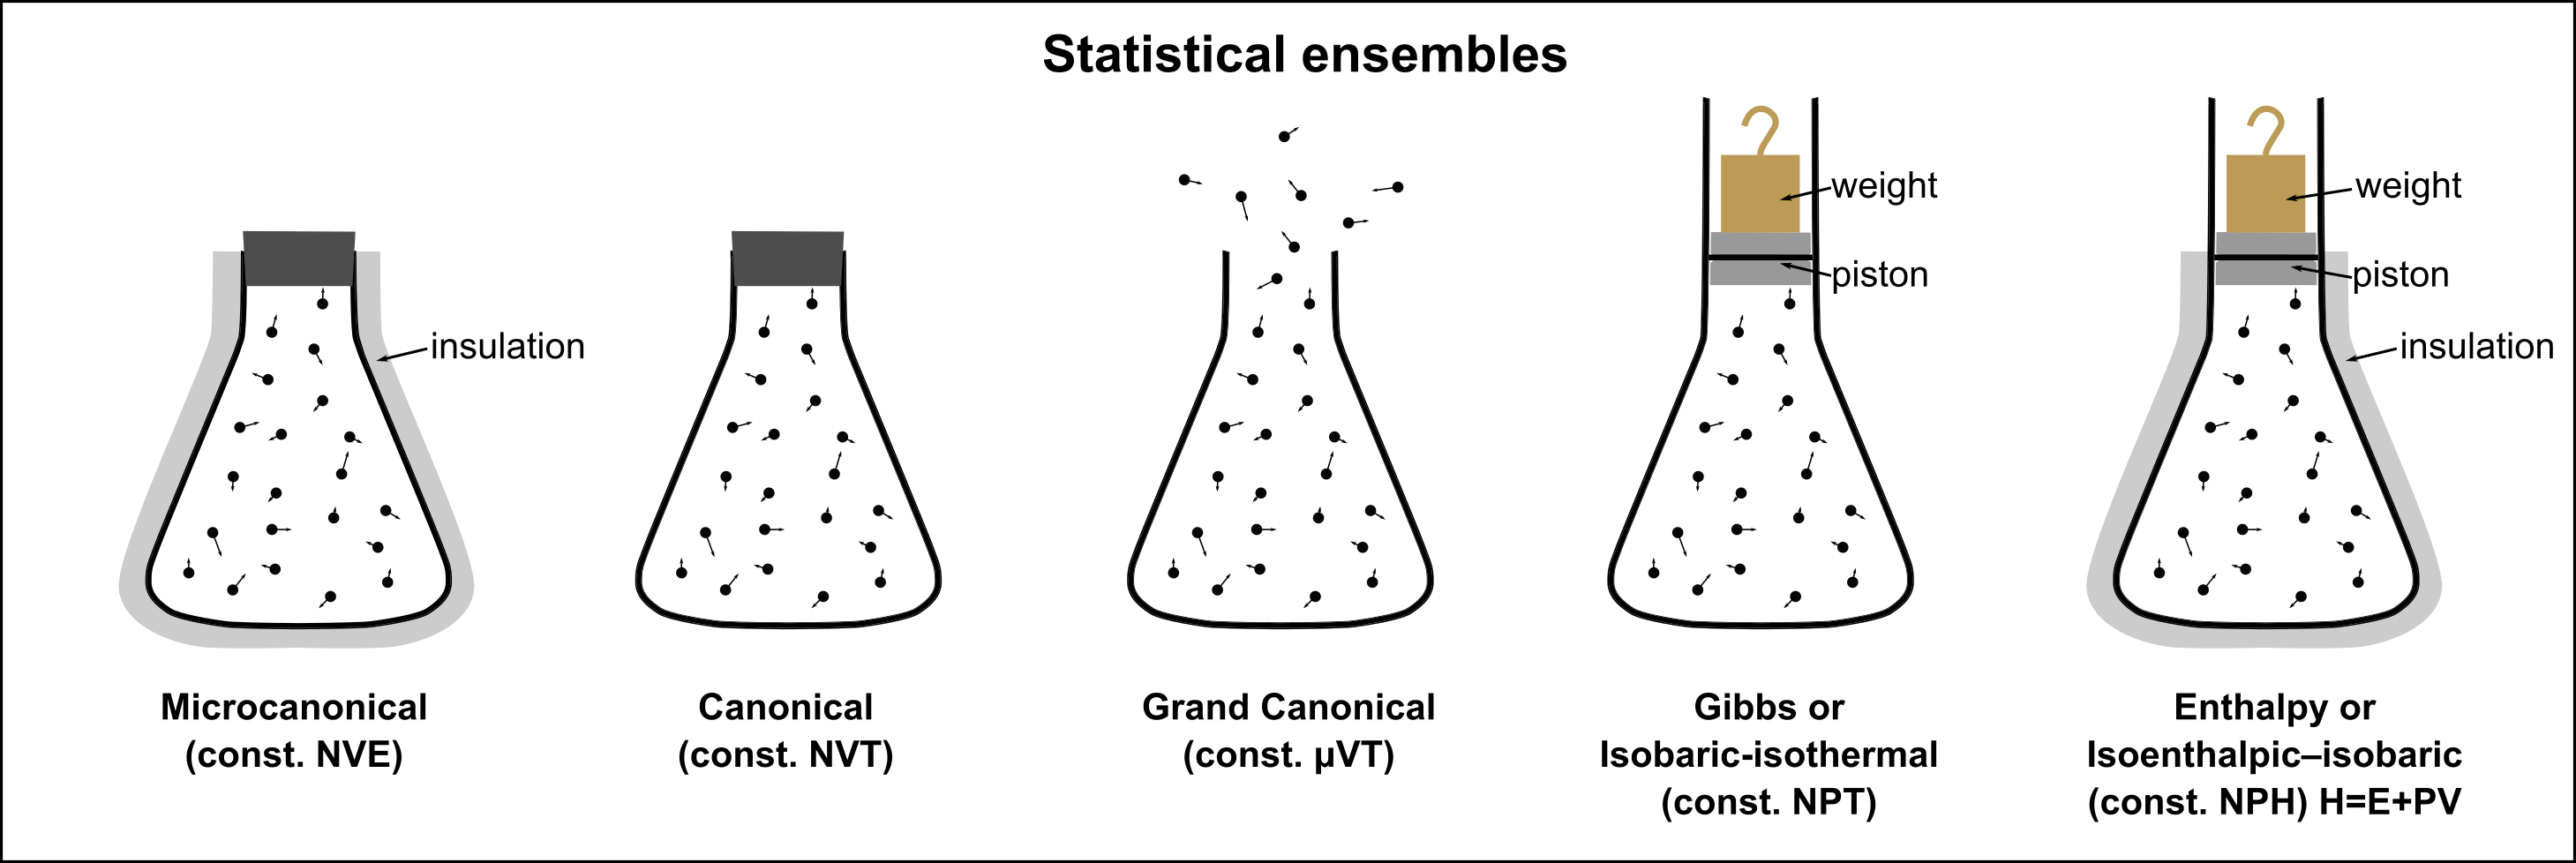
\includegraphics[height=1.20in,width=3.75in,viewport=0 0 1420 470,clip]{Figures/Statistical_Ensembles.png}
\caption{\tiny \textrm{The Statistical Ensembles.}}%(与文献\cite{EPJB33-47_2003}图1对比)
\label{Statistical_Ensembles}
\end{figure}
\vskip -15pt
\begin{itemize}
		{\fontsize{7.2pt}{1.2pt}\selectfont{
		\item 微正则系综\textrm{(Mircocanonical Ensemble)}\footnote{\fontsize{4.5pt}{1.2pt}\selectfont{\textrm{canonical},汉译作“正则”,出自《楚辞\textperiodcentered 离骚》“皇揽揆余於初度兮,肇锡余以嘉名;~名余曰\textcolor{red}{正则}兮,字余曰灵均”,《楚辞章句》\upcite{Chucizhangju}:~“正,平也;~则,法也;~灵,神也;~均,调也。言正平可法则者,莫过于天;~养物均调者,莫神于地。高平曰原,故父伯庸名我为平以法天,字我为原以法地。言己上之能安君,下之能养民也。”,意思是说“正则”、“灵均”隐喻着某种意义,即平正是天的象征,原均是地的象征。因此正则的含义是“\textcolor{blue}{符合天道}”,与\textrm{canonical}的意思\textrm{of, relating to, or forming a canon}意义一致。}}:~\textrm{NVE}皆为常数
		\item 正则系综\textrm{(Canonical Ensemble)}:~\textrm{NVT}皆为常数
		\item 巨正则系综\textrm{(Grandcanonical Ensemble)}:~\textrm{$\mu$VT}皆为常数,粒子数不固定
		\item 等压-等温系综\textrm{(Isobaric-Isothermal Ensemble)}:~\textrm{NPT}皆为常数
		\item 等焓-等压系综\textrm{(Isoenthalpic-Isobaric Ensemble)}:~\textrm{NPH}皆为常数
		\item 等张力-等温系综\textrm{(Isotension-Isothermal Ensemble)}:~容器形状可变 }}
\end{itemize}
}

\frame
{
	\frametitle{常用热力学量}
	\begin{itemize}
{\fontsize{7.8pt}{1.2pt}\selectfont{
		\item 动能 ~$E_{\mathrm{k}}=\bigg\langle\sum\limits_{i=1}^N\dfrac12m_iv_i^2\bigg\rangle$
		\item 势能 ~$E_{\mathrm{p}}=\bigg\langle\sum\limits_{i=1}^NE_{\mathrm{p}i}\bigg\rangle$
		\item 温度 ~$T=\dfrac1{\mathrm{d}Nk_{\mathrm{B}}}\bigg\langle\sum\limits_{i=1}^Nm_iv_i^2\bigg\rangle$ ~~~~ 其中$\mathrm{d}$是空间维度
		\item 压强 ~$p=\dfrac{k_{\mathrm{B}}TN}{V}+\dfrac1{\mathrm{d}V}\bigg\langle\sum\limits_{i<j}\vec f_{ij}\cdot\vec r_{ij}\bigg\rangle$
		\item 焓 ~$H=E+pV$ ~~~~ 相当于\textrm{NPT}下的有效总内能
		\item 熵 ~$S=k_{\mathrm{B}}\ln\Omega(N,V,E)$ ~~~~ $\Omega$是系统的总的微观状态数
		\item \textrm{Helmholtz}自由能:~\textcolor{blue}{\textrm{NVT}下的自由能}
			\begin{displaymath}
				F=E-TS=-k_{\mathrm{B}}T\ln{Q}
			\end{displaymath}
		\item \textrm{Gibbs}自由能:~\textcolor{blue}{\textrm{NPT}下的自由能}
			\begin{displaymath}
				G=F+pV=E-TS+pV
			\end{displaymath}
		\item 化学势 ~$\mu=\dfrac{\partial G}{\partial N}\bigg|_{T,p}=\dfrac{\partial F}{\partial N}\bigg|_{T,V}$}}
	\end{itemize}
}

\subsection{采样与模拟}
\frame
{
	\frametitle{空间、边界与周期边界条件}
	\begin{itemize}
		\item 空间的连续性
			\vskip 2pt
			{\fontsize{8.5pt}{1.2pt}\selectfont{离散模型:~如\textrm{Ising}模型\\
			连续模型 }}
		\item 边界条件:~自由、刚性、周期
	\end{itemize}
	\textcolor{blue}{周期边界条件}\textrm{(Periodic Boundary Condition, PBC)}\\
	\begin{itemize}
		\item \textcolor{blue}{目标}:~少量分子或团簇$(10^3\sim10^6)$的模拟与含有大量宏观粒子体系$(\sim10^{23})$
		\item \textcolor{blue}{策略}:~模拟的容器中粒子与无穷多镜像中粒子存在相互作用
	\end{itemize}
	\begin{displaymath}
		\begin{aligned}
			\vec F_{\mathrm{PBC}}(\vec r_i-\vec r_j)=&\sum_n\vec F\bigg(\bigg|\vec r_i-\vec r_j+\sum_{\mu=1}^3\mathbf{L}_{\mu}n_{\mu}\bigg|\bigg)\\
			E_{\mathrm{tot}}=&\dfrac12\sideset{}{^{\prime}}\sum_{i,j,n}\varepsilon\big(\big|\vec r_{ij}+n\mathbf{L}\big|\big)
		\end{aligned}
	\end{displaymath}
}

\frame
{
	\frametitle{空间、边界与周期边界条件}
\begin{figure}[h!]
\centering
\vspace*{-0.15in}
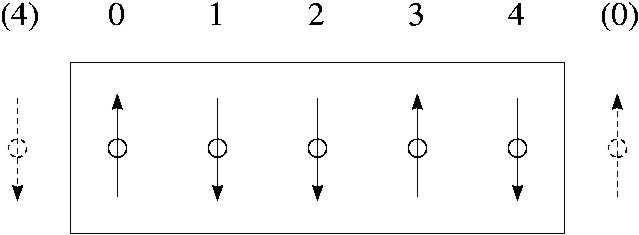
\includegraphics[height=0.75in,width=2.35in,viewport=0 0 460 170,clip]{Figures/Periodic-boundary-conditions-on-a-spin-lattice.jpg}
\vskip 1pt
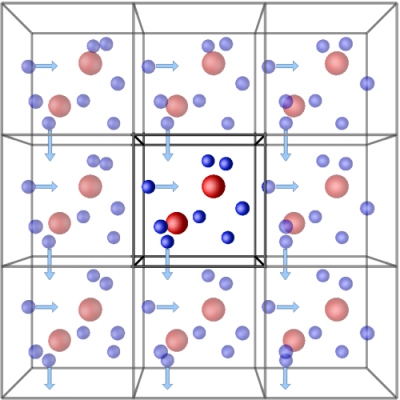
\includegraphics[height=1.95in,width=2.15in,viewport=0 0 300 300,clip]{Figures/Periodic-boundary-conditions.png}
\caption{\tiny \textrm{Schematic representation of the idea of periodic boundary conditions.}}%(与文献\cite{EPJB33-47_2003}图1对比)
\label{Periodic_boundary_conditions}
\end{figure}
}

\frame
{
	\frametitle{模拟与采样参数}
	\begin{itemize}
		\item \textcolor{blue}{特征长度}\textrm{(characteristic length)}:~物理量在空间的相关长度\\
			{\fontsize{8.5pt}{1.2pt}\selectfont{原则上,模拟容器的边长应大于关心物理量的特征长度;~具体操作上,可以通过变化模拟尺寸来了解有限尺寸效应\textrm{(finite size effect)}的影响}}
		\item \textcolor{blue}{截断距离}\textrm{(cutoff distance)}:~应小于模拟容器边长的一半\\
			{\fontsize{8.5pt}{1.2pt}\selectfont{避免同一粒子与两个镜像同时作用;~截断的处理方式有:~简单截断、截断平移、最小镜像法等三种}}
		\item \textcolor{blue}{采样}\textrm{(sampling)}:~本质是有限时间内的重要性采样\textrm{(importance sampling)}\\
			{\fontsize{8.5pt}{1.2pt}\selectfont{采样对系综平均贡献最大的瞬时量的子集,一般采用均匀时间间隔采样}}
		\item \textcolor{blue}{初始构型}\textrm{(Initial Configuration)}:~要尽量接近平衡态\\
			{\fontsize{8.5pt}{1.2pt}\selectfont{一般需要一定的初始模拟过程使得初始构型达到平衡态,在此初始模拟过程中不采样,需要根据某些参数的变化观察系统是否达到平衡态(液体体积很容易平衡,势能次之,扩散系数较难达到平衡)}}
		\item \textcolor{blue}{样本相关度}\textrm{(Correlation)}:~离得越近采样样本相关度越大\\
			{\fontsize{8.5pt}{1.2pt}\selectfont{相关的样本不影响平均值,但会影响误差范围}}
	\end{itemize}
}

\frame
{
	\frametitle{\textrm{Maxwell-Boltzmann}分布}
\begin{figure}[h!]
\centering
\vspace*{-0.15in}
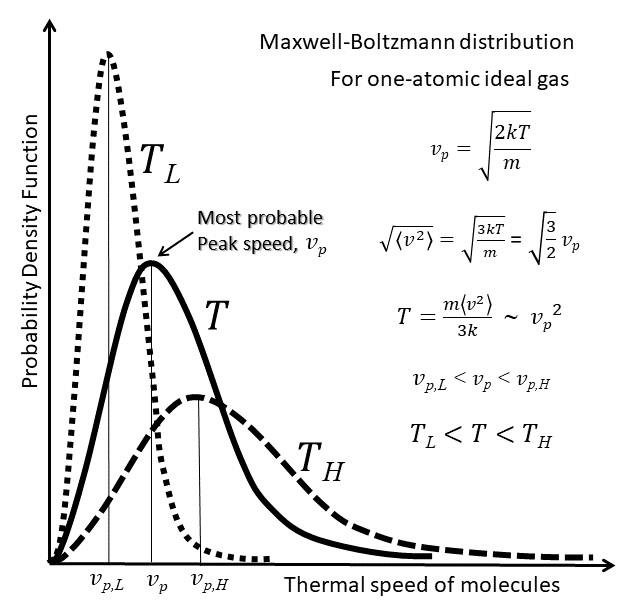
\includegraphics[height=2.75in,width=3.25in,viewport=0 0 470 460,clip]{Figures/Maxwell-Boltzmann-distribution-Energetic-molecules-of-an-ideal-gas.jpeg}
%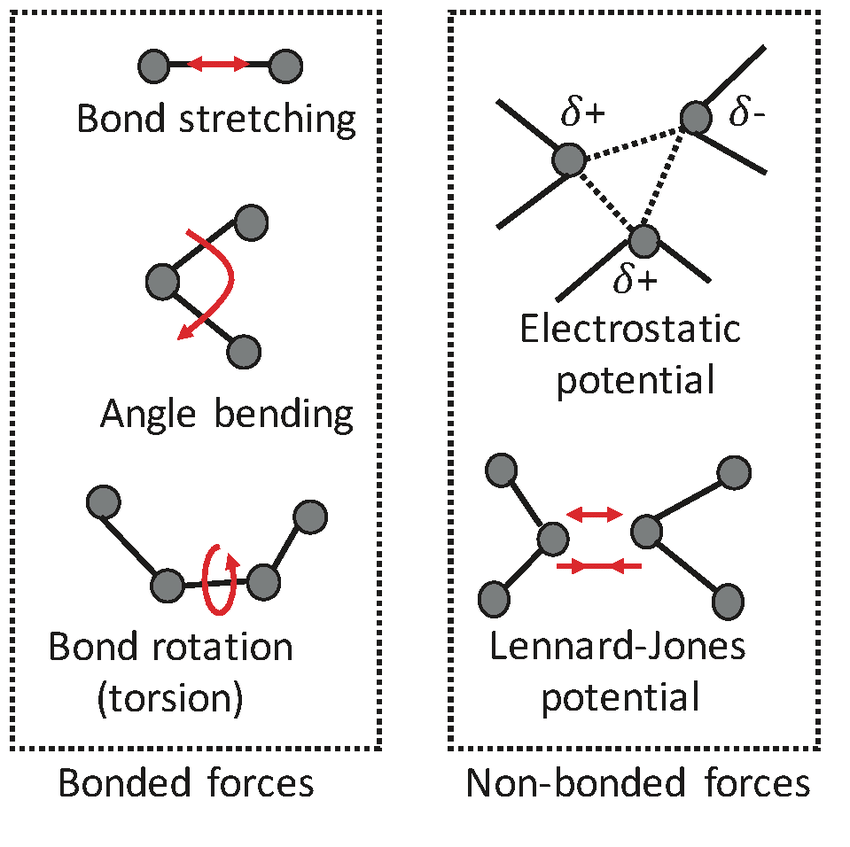
\includegraphics[height=2.70in,width=2.85in,viewport=0 40 830 850,clip]{Figures/Bonded-and-non-bonded-forces-consider-in-MD-simulations.png}
\caption{\tiny \textrm{Maxwell-Boltzmann distribution Energetic molecules of an ideal gas.}}%(与文献\cite{EPJB33-47_2003}图1对比)
\label{Maxwell-Boltzmann-distribution}
\end{figure}
}

\frame
{
	\frametitle{热耦或热浴\textrm{(Thermostat or Heat~Bath)}}
	\begin{itemize}
		\item \textrm{Isokinetics thermostat}:\\
			每一步采样都对速度进行修正,直到体系达到设定的目标温度
			\begin{displaymath}
				\dfrac32Nk_{\mathrm{B}}T=\dfrac12\sum_im_iv_i^2\Longrightarrow v_i^{\mathrm{scale}}=\lambda v_i\quad\mbox{有}~\lambda=\sqrt{\dfrac{T}{T_0}}
			\end{displaymath}
		\item \textrm{Berendsen thermostat}:
			\begin{displaymath}
				\lambda=\bigg[1+\dfrac{\Delta t}{\tau_T}\bigg(\dfrac{T}{T_0}-1\bigg)\bigg]^{\frac12}
			\end{displaymath}
		\item \textrm{Andersen thermostat}:\\
			每一步从温度为$T$的\textrm{Maxwell-Boltzmann}分布中随机产生一个速度赋予被选中的粒子
		\item \textrm{Nos\'e-Hoover thermostat}:\\
			增加额外的自由度,在扩展的微正则系综内实现实际体系的正则系综
	\end{itemize}
}

\frame
{
	\frametitle{离子间相互作用的\textrm{Ewald}求和}
	周期边界下长程\textrm{Coulomb}相互作用的计算\\
	通过屏蔽电荷将点电荷分解为时空间中的长程部分和短程部分
	\begin{itemize}
		\item \textcolor{blue}{短程部分}:~实空间截断
		\item \textcolor{blue}{长程部分}:~$\vec k$-空间截断
	\end{itemize}
\begin{figure}[h!]
\centering
%\vspace*{-0.20in}
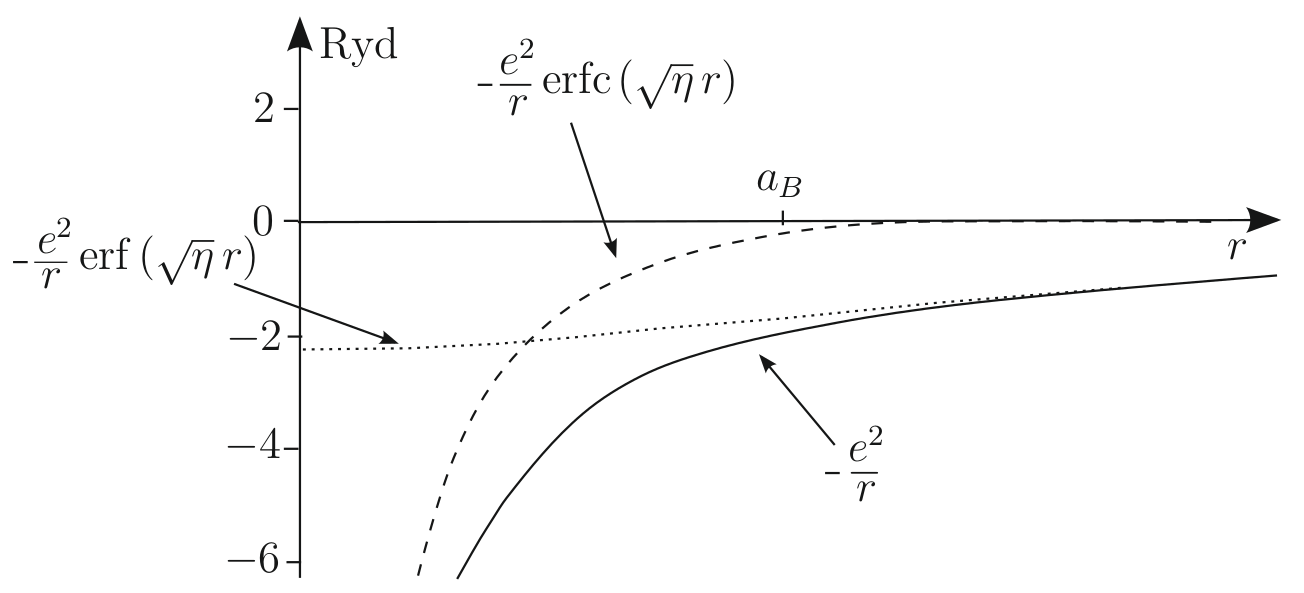
\includegraphics[height=1.2in,width=2.82in,viewport=0 0 1100 455,clip]{Figures/Ewald_method.png}
\caption{\fontsize{5.5pt}{2.2pt}\selectfont{\textrm{Decomposition of the potential $-e^2/r$ (singular at the origin and of long-range nature) into a contribution $-(e^2/r)\mathrm{erf}(\sqrt{\eta}r)$(regular at the origin of long-range) and a contribution $-(e^2/r)\mathrm{erfc}(\sqrt{\eta}r)$ (singular at the origin and of short-range nature). Here $\sqrt{\eta}=1 (\mathrm{Bohr radius unit})$ is chosen.}}}%(与文献\cite{EPJB33-47_2003}图1对比)
\label{Error_Function}
\end{figure}
}

\frame
{
	\frametitle{离子间相互作用的\textrm{Ewald}求和}
\begin{figure}[h!]
\centering
\vspace*{-0.20in}
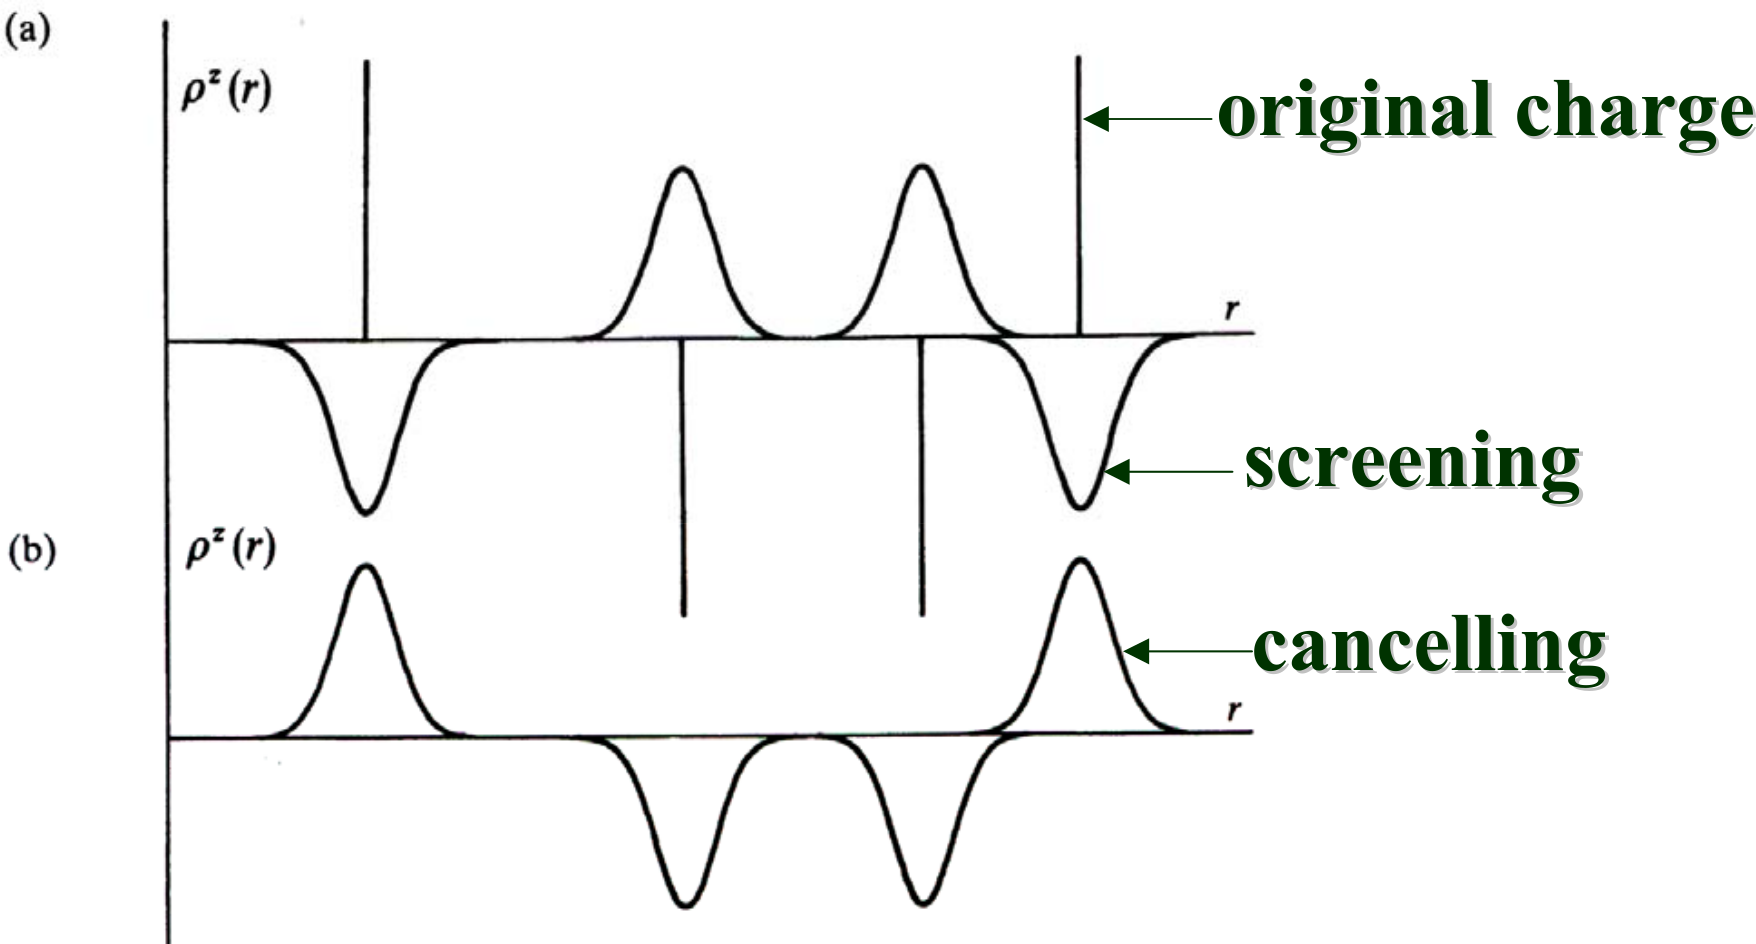
\includegraphics[height=1.6in,width=3.32in,viewport=0 0 1800 955,clip]{Figures/Ewald_method-2.png}
\caption{\fontsize{5.5pt}{2.2pt}\selectfont{\textrm{Each charge be screened by a Gaussian charge distribution of opposite sign and equal magnitude: $\rho_i(r)=\dfrac{Z_i\eta^3}{\pi^{3/2}}\mathrm{e}^{-\eta^2r^2}$.}}}%(与文献\cite{EPJB33-47_2003}图1对比)
\label{Ewald_method-2}
\end{figure}
\textrm{Particle mesh Ewald~(PME)}和\textrm{Particle-Particle Particle-Mesh~(PPPM)}算法:\\
空间离散化,应用快速\textrm{Fourier}变换\textrm{(Fast Fourier Transform, FFT)}将计算复杂度由$\mathscr{O}(N^2)$降为$\mathscr{O}(N\log(N))$
}

\frame
{
	\frametitle{邻居列表\textrm{(neighbour list)}}
	\begin{itemize}
		\item 遍历模拟体系全部任意两个粒子间距离的计算复杂度为$\mathscr{O}(N^2)$,实际计算中,对于短程相互作用,可以忽略远距离的长程作用,截断后的计算复杂度将大大下降
		\item \textcolor{blue}{\textrm{The minimum-image convention}}:\\为加速计算,将容器空间划分成小的立方体\textrm{(cell)},每个\textrm{cell}的边长为截断距离。计算粒子距离时,对于给定粒子只须遍历最近邻27个\textrm{cell}内的粒子(包括本身所在的\textrm{cell})。计算复杂度降为$\mathscr{O}(N)$
\begin{figure}[h!]
\centering
\vspace*{-0.18in}
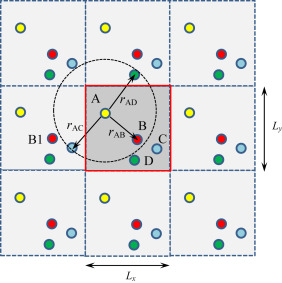
\includegraphics[height=1.2in,width=1.28in,viewport=0 0 180 180,clip]{Figures/Schematic-showing-the-closest-neighbors-of-atom_A-in-the-primary-simulation-cell-as-determined-by-the-minimum-image-criterion.jpg}
\caption{\fontsize{5.5pt}{2.2pt}\selectfont{\textrm{Schematic showing the closest neighbors of atom A in the primary simulation cell as determined by the minimum image criterion.}}}%(与文献\cite{EPJB33-47_2003}图1对比)
\label{Minimum-image-convention}
\end{figure}
	\end{itemize}
	
}

\subsection{数据分析}
\frame
{
	\frametitle{能量数据}
	\begin{itemize}
		\item 总能量~$E=E_{\mathrm{k}}+E_{\mathrm{p}}$
\begin{displaymath}
	\begin{aligned}
		E_{\mathrm{k}}=&\bigg\langle\sum\limits_{i=1}^N\dfrac12m_iv_i^2\bigg\rangle\\
		E_{\mathrm{p}}=&\bigg\langle\sum\limits_{i=1}^NE_{\mathrm{p}i}\bigg\rangle 
	\end{aligned}
\end{displaymath}
\item 比热容~$C_V^{\mathrm{NVT}}=\dfrac{\big\langle E_{\mathrm{p}}^2\big\rangle-\big\langle E_{\mathrm{p}}\big\rangle^2}{k_{\mathrm{B}}T^2}+\dfrac32Nk_{\mathrm{B}}$
\item 瞬时温度 ~$T=\dfrac2{\mathrm{d}Nk_{\mathrm{B}}}E_{\mathrm{k}}$ ~~~~ 其中$\mathrm{d}$是空间维度
\item 瞬时压强 ~$P=\rho k_{\mathrm{B}}T+\dfrac1{\mathrm{d}V}\bigg\langle\sum\limits_{i<j}\vec f_{ij}(\vec r_{ij})\cdot\vec r_{ij}\bigg\rangle$
	\end{itemize}
}

\frame
{
	\frametitle{相关系数}
	\begin{displaymath}
		\begin{aligned}
			c(A,B)&=\dfrac{\big\langle\big(A-\langle A\rangle\big)\big(B-\langle B\rangle\big)\big\rangle}{\sqrt{\big\langle\big(A-\langle A\rangle\big)^2\big\rangle\big\langle\big(B-\langle B\rangle\big)^2\big\rangle}}\\
			c&\in[0,1]
		\end{aligned}
	\end{displaymath}
	\begin{itemize}
		\item 时间相关系数\\
			\begin{displaymath}
				c(A,B,t)=\dfrac{\big\langle\big(A(t+t_0)-\langle A(t+t_0)\rangle\big)\big(B(t_0)-\langle B(t_0)\rangle\big)\big\rangle}{\sqrt{\big\langle\big(A(t+t_0)-\langle A(t+t_0)\rangle\big)^2\big\rangle\big\langle\big(B(t_0)-\langle B(t_0)\rangle\big)^2\big\rangle}}
			\end{displaymath}
		\item 时间自相关系数
			\begin{displaymath}
				c(A,t)=\dfrac{\big\langle\big(A(t+t_0)-\langle A(t+t_0)\rangle\big)\big(A(t_0)-\langle A(t_0)\rangle\big)\big\rangle}{\big\langle\big(A(t_0)-\langle A(t_0)\rangle\big)^2\big\rangle}
			\end{displaymath}
	\end{itemize}
}

\frame[allowframebreaks]
{
	\frametitle{结构特征}
	\begin{itemize}
		\item \textrm{Radial distribution function~(RDF)}:\\
			在距离$r$处找到粒子的概率
			\begin{displaymath}
				g(r)=\dfrac{V}{N^2}\bigg\langle\sum_i\sum_{j\neq i}\delta(\vec r-\vec r_{ij})\bigg\rangle
			\end{displaymath}
			理想气体~$g(r)=1$

\begin{figure}[h!]
\centering
\vspace*{-0.15in}
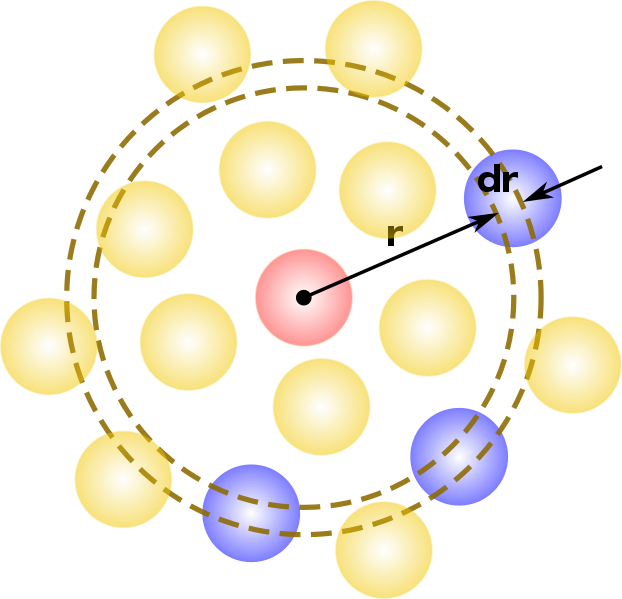
\includegraphics[height=1.0in,width=1.1in,viewport=0 0 630 600,clip]{Figures/Rdf_schematic.png}
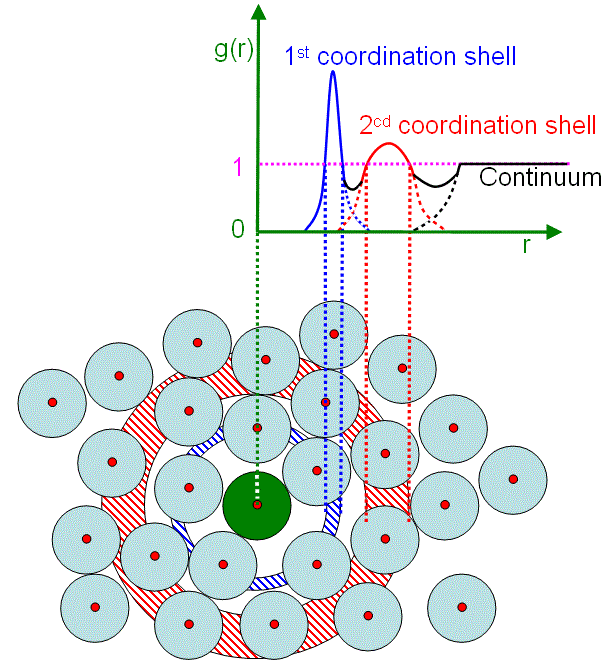
\includegraphics[height=1.0in,width=0.9in,viewport=0 0 610 660,clip]{Figures/Schematic-illustration-of-g(r)-dependence-on-r.png}
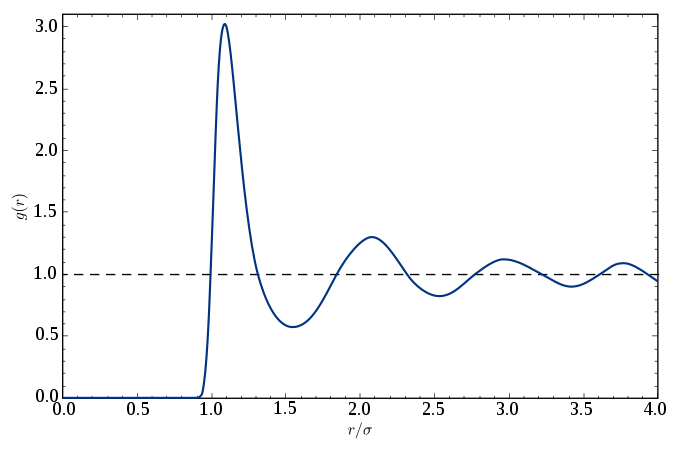
\includegraphics[height=1.0in,width=1.6in,viewport=0 0 680 480,clip]{Figures/Lennard-Jones_Radial_Distribution_Function.png}
\caption{\fontsize{5.5pt}{2.2pt}\selectfont{\textrm{Schematic illustration of g(r) dependence on r and the radial distribution function for Lennard-Jones fluid at $T^{\ast}=0.71$, $n^{\ast}=0.844$.}}}%(与文献\cite{EPJB33-47_2003}图1对比)
\label{Radial_distribution-function}
\end{figure}
		\item \textrm{Structure factor}:\\
			\textrm{RDF}在$\vec k$空间的\textrm{Fourier}变换,实验可直接观测的物理量
			\begin{displaymath}
				S(k)=1+4\pi\rho\int_0^{\infty}r^2\dfrac{\sin(\vec k\cdot\vec r)}{\vec k\cdot\vec r}g(r)\mathrm{d}r
			\end{displaymath}
\begin{figure}[h!]
\centering
\vspace*{-0.25in}
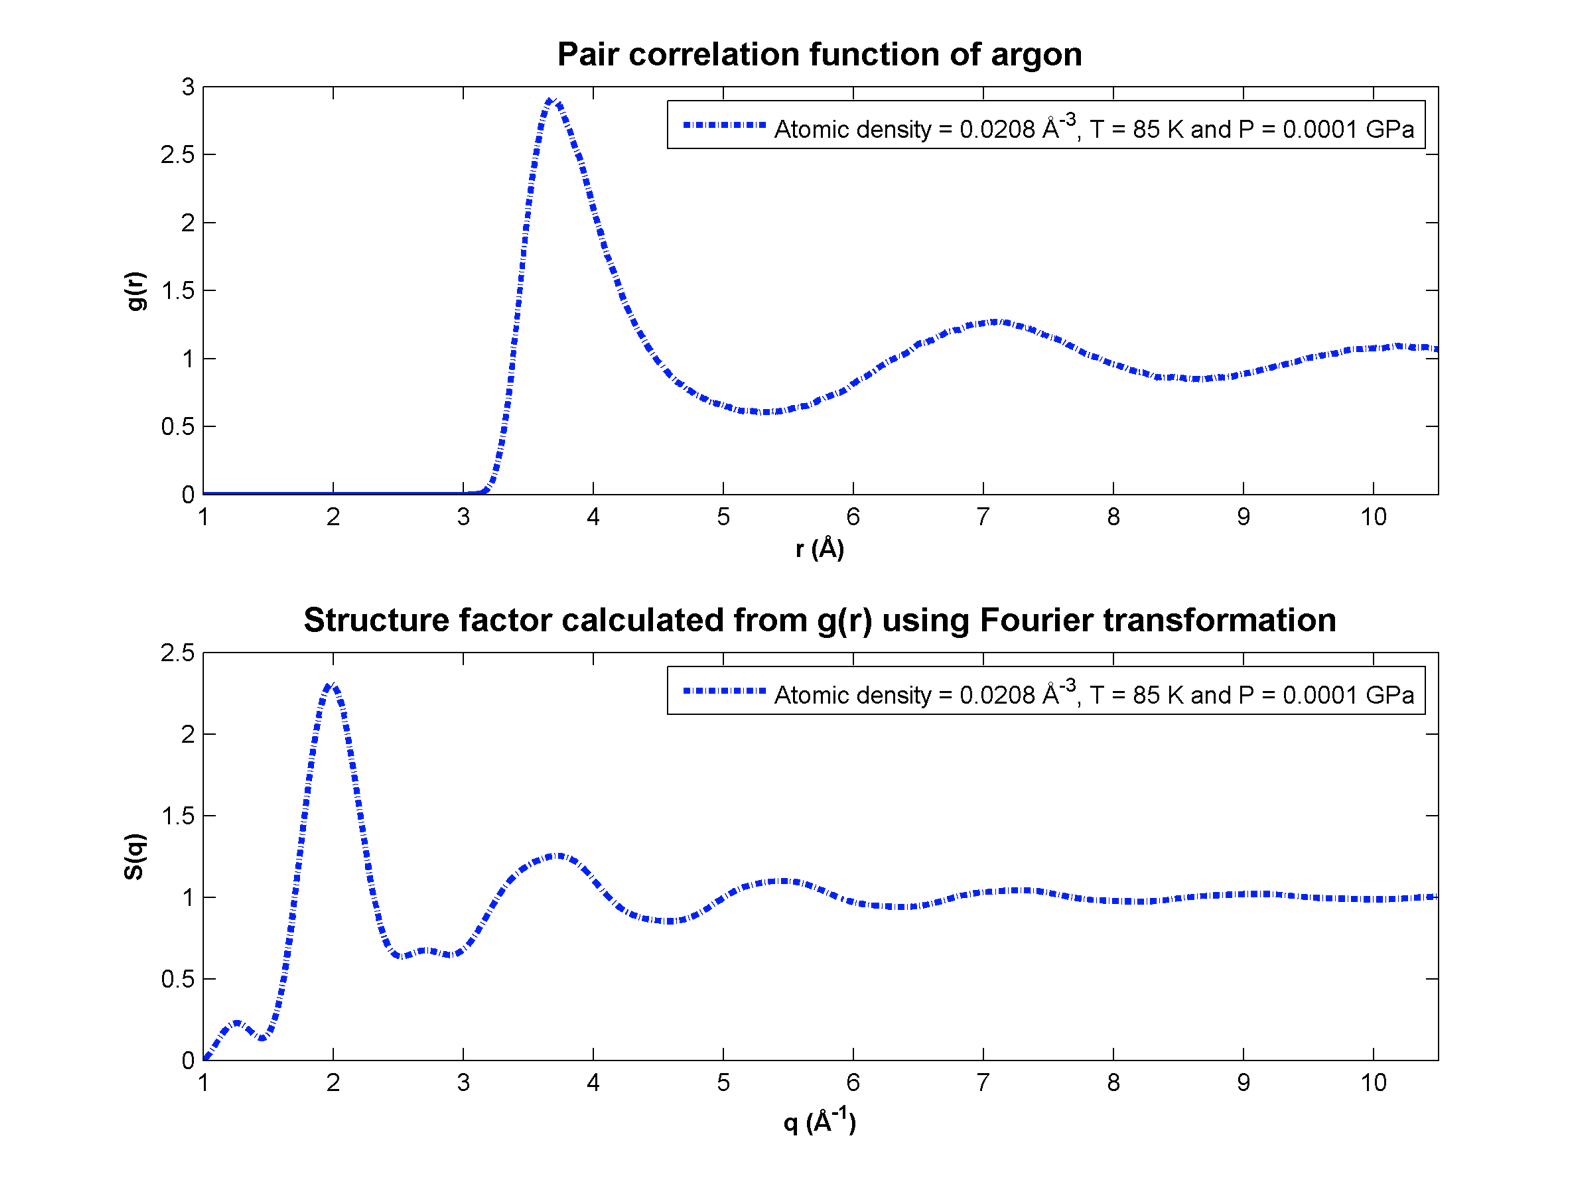
\includegraphics[height=1.4in,width=1.9in,viewport=60 10 730 580,clip]{Figures/Structure-factor-RDF.png}
\caption{\fontsize{5.5pt}{2.2pt}\selectfont{\textrm{The structure factor of argon calculating from a radial distribution function.}}}%(与文献\cite{EPJB33-47_2003}图1对比)
\label{Structure-factor}
\end{figure}
	\end{itemize}
}

\frame
{
	\frametitle{扩散系数}
	\begin{itemize}
		\item \textrm{Mean square displacement~(MSD)}:\\
			时间$t$间隔内粒子运动的平均距离的平方
			\begin{displaymath}
				\big\langle r^2(t)\big\rangle\equiv\big\langle\Delta r^2(t)\big\rangle=\dfrac1N\sum_{i=1}^N\Delta r_i^2(t)
			\end{displaymath}
		\item \textrm{Diffusion coefficient}:\\
			\begin{displaymath}
				\big\langle r^2(t)\big\rangle=2\mathrm{d}D\qquad\qquad \mbox{\textrm{d}是空间维度}
			\end{displaymath}
			\item \textrm{Velocity autocorelation function~(VACF)}:\\
				\begin{displaymath}
					\begin{aligned}
						&\big\langle\vec v(t)\vec v(0)\big\rangle\\
						D=&\int_0^{\infty}\langle\vec v(t)\vec v(0)\mathrm{d}t
					\end{aligned}
				\end{displaymath}

	\end{itemize}
}

\frame
{
	\frametitle{扩散系数}
\begin{figure}[h!]
\centering
\vspace*{-0.2in}
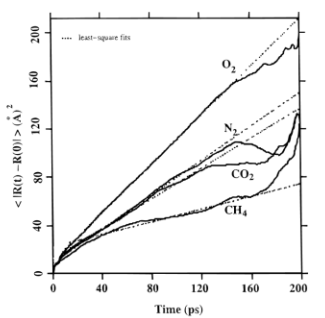
\includegraphics[height=1.2in,width=2.0in,viewport=0 0 350 300,clip]{Figures/MSD_O2-N2-CO2-CH4.png}\\
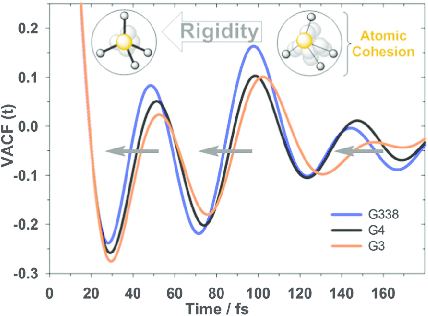
\includegraphics[height=1.6in,width=2.8in,viewport=0 0 230 160,clip]{Figures/The-velocity-autocorrelation-function-VACF-of-the-Al-atoms-showing-the-increase-of-rigidity of the local Al-coordination-for-G3-G4-and-G338-glasses.png}
%\caption{\fontsize{5.5pt}{2.2pt}\selectfont{\textrm{The structure factor of argon calculating from a radial distribution function.}}}%(与文献\cite{EPJB33-47_2003}图1对比)
\label{MSD-VACF}
\end{figure}
}

\section{\rm{LAMMPS}软件基础}
\frame
{
	\frametitle{\textrm{LAMMPS}简介}
	\textcolor{blue}{\textrm{LAMMPS}}:\\
	\textrm{Large-scale Atomic/Molecular Massively Parallel Simulator}\\
	美国能源部的两个实验室和三个公司联合开发\\
	由\textrm{Sandia}国家实验室发布
	\begin{itemize}
			\setlength{\itemsep}{10pt}
		\item 固态、液态、气态的经典分子动力学模拟
		\item 易于扩展:~方便引入新的力场、原子类型和边界条件
		\item 开发语言:~\textrm{C++-MPI/FFT}
		\item 支持\textrm{GPU}计算,支持\textrm{OpenMP}
		\item 脚本可支持一个或多个模拟进程
	\end{itemize}
}

\frame
{
	\frametitle{模型\textrm{(atom\_style)}}
	\begin{itemize}
		\item 原子或简单分子
		\item 粗粒化粒子~(如有机高分子模型:~小球-弹簧模型)
		\item \textrm{United-atom}高分子或有机分子
		\item 全原子高分子:~有机分子、蛋白质、\textrm{DNA}
		\item 金属:~金属单质、合金
		\item 颗粒物质
		\item 粗粒化介观模型
		\item 有限尺度球和椭球粒子
		\item 有限尺度\textrm{line segment~(2d)}与三角\textrm{(3d)}粒子
		\item 偶极粒子
		\item 硬球粒子
		\item 上述模型的组合
	\end{itemize}
}

\frame[allowframebreaks]
{
	\frametitle{各类力场}
	\begin{itemize}
{\fontsize{9.5pt}{2.2pt}\selectfont{
		\item \textcolor{blue}{二体势}:~\textrm{Lennard-Jones, Buckingham, Morse, Born-Mayer-Huggins, Yukawa, soft, COMPASS,hydrogen bond, tabulated}
		\item \textcolor{blue}{带点二体势}:~\textrm{Coulomb}势,点电荷-电偶极矩作用
		\item \textcolor{blue}{多体势}:~\textrm{EAM, Finnis/Sinclair EAM, modified EAM~(MEAM), embedded ion method~(EIM), EDIP, ADP, Stillinger-Weber, Tersoff, REBO, AIREBO, ReaxFF, COMB}
		\item \textcolor{blue}{电子力场}:~\textrm{eFF, AWPMD}
		\item \textcolor{blue}{粗粒化势}:~\textrm{DPD, GayBerne, REsquared, colloidal, DLVO}
		\item \textcolor{blue}{介观势}:~\textrm{granular, Peridynamics, SPH}
		\item \textcolor{magenta}{Bond potentials}:~\textrm{harmonic, FENE, Morse, nonlinear, class 2, quartic (breakable)}
		\item \textcolor{magenta}{Angle potentials}:~\textrm{harmonic, CHARMM, cosine, cosine/squared, cosine/periodic, class 2~(COMPASS)}
		\item \textcolor{magenta}{Dihedral potentials}:~\textrm{harmonic, CHARMM, multi-harmonic, helix, class 2~(COMPASS), OPLS}
		\item \textcolor{magenta}{Improper potentials}:~\textrm{harmonic, cvff, umbrella, class 2~(COMPASS)}
		\item \textcolor{purple}{高分子势}:~\textrm{all-atom, united-atom,bead-spring, breakable}
		\item \textcolor{purple}{水分子势}:~\textrm{TIP3P, TIP4P, SPC}
		\item \textcolor{purple}{隐含溶液势}:~\textrm{hydrodynamic lubrication, Debye}
		\item \textcolor{blue}{\textrm{KIM archive of potentials}}
		\item \textcolor{purple}{长程势}:~\textrm{Ewald, Wolf, PPPM~(similar to particle-mesh Ewald), Ewald/N for long-range Lennard-Jones}
		\item 与常用力场\textrm{CHARMM, AMBER, DREIDING, OPLS, GROMACS, COMPASS}格式兼容}}
	\end{itemize}
}

\frame
{
	\frametitle{初始构型}
	\begin{itemize}
		\item 
	\end{itemize}<++>
}

%------------------------------------------------------------------------Reference----------------------------------------------------------------------------------------------
		\frame[allowframebreaks]
{
\frametitle{主要参考文献}
\begin{thebibliography}{99}
{\tiny
	\bibitem{JCP27-1208_1957}\textrm{B.J. Alder, T.E. Wainwright. \textit{J. Chem. Phys.} \textbf{27} (1957), 1208}
	\bibitem{Comp_Phys}\textrm{J. M. Thijssen. \textit{Computational Physics (2nd Edition)} (Cambridge University Press, Cambridge, England, 2007)}
	\bibitem{Lammps_turtorial}王延颋, \textrm{LAMMPS}教程~中科院超算中心培训, 北京, \textrm{2012}
	\bibitem{Chucizhangju}[东汉]王逸\:撰,黄灵庚\:点校, {\textit{楚辞章句}}\:上海古籍出版社, 上海, \textrm{2017}
}
\end{thebibliography}
%\nocite*{}
}
